\documentclass[dissertation,CC-BY-ND]{uathesis}


\usepackage[a4paper,width=150mm,top=25mm,bottom=25mm]{geometry}
\usepackage[T1]{fontenc}
\usepackage[utf8]{inputenc}
\usepackage{authblk}
\usepackage{graphicx}
\usepackage{natbib}
%\usepackage{chapterbib}
\usepackage[cmex10]{amsmath}
\usepackage{amssymb}
\usepackage{amsthm}
\usepackage{mathrsfs}
\usepackage{hyphenat}
\usepackage{url}
\usepackage{listings}
\usepackage{color}

\definecolor{dkgreen}{rgb}{0,0.6,0}
\definecolor{gray}{rgb}{0.5,0.5,0.5}
\definecolor{mauve}{rgb}{0.58,0,0.82}

\lstset{frame=tb,
  language=Python,
  aboveskip=3mm,
  belowskip=3mm,
  showstringspaces=false,
  columns=flexible,
  basicstyle={\small\ttfamily},
  numbers=none,
  numberstyle=\tiny\color{gray},
  keywordstyle=\color{blue},
  commentstyle=\color{dkgreen},
  stringstyle=\color{mauve},
  breaklines=true,
  breakatwhitespace=true,
  tabsize=3
}

\usepackage[bookmarks,colorlinks=true,urlcolor=black,linkcolor=black,citecolor=black]{hyperref}
\usepackage{cleveref}
\crefname{section}{Section}{Sections}
\crefname{figure}{Figure}{Figures}
\crefname{table}{Table}{Tables}
\setcounter{secnumdepth}{3} 
\setcounter{tocdepth}{3}

\newcommand{\Tmat}{\textbf{T}}
\newcommand{\vvec}{\textbf{v}}
\newcommand{\meanvvec}{\overline{\vvec}}
\newcommand{\delmeanvvec}{\Delta \meanvvec}
\newcommand{\vnhvec}{\boldsymbol{v_0}}
\newcommand{\vonevec}{\boldsymbol{v_1}}
\newcommand{\vtwovec}{\boldsymbol{v_2}}

\newcommand{\gvec}{\textbf{g}}
\newcommand{\meangvec}{\overline{\gvec}}
\newcommand{\delmeangvec}{\Delta \meangvec}
\newcommand{\gnhvec}{\boldsymbol{g_0}}
\newcommand{\gonevec}{\boldsymbol{g_1}}
\newcommand{\gtwovec}{\boldsymbol{g_2}}

\newcommand{\fvec}{\textbf{f}}
\newcommand{\xvec}{\textbf{x}}
\newcommand{\nvec}{\textbf{n}}
\newcommand{\rvec}{\textbf{r}}
\newcommand{\pvec}{\textbf{p}}
\newcommand{\Hmat}{\textbf{H}}
\newcommand{\Xvec}{\textbf{X}}
\newcommand{\Wvec}{\textbf{W}}

\newcommand{\Wv}{\textbf{W}_\textbf{v}}
\newcommand{\Wg}{\textbf{W}_\textbf{g}}
\newcommand{\WH}{\textbf{W}_\textbf{H}}

\newcommand{\Kv}{\textbf{K}_\textbf{v}}
\newcommand{\Kg}{\textbf{K}_\textbf{g}}
\newcommand{\Kx}{\textbf{K}_\textbf{x}}
\newcommand{\Kone}{\textbf{K}_\textbf{1}}
\newcommand{\Ktwo}{\textbf{K}_\textbf{2}}
\newcommand{\Kj}{\textbf{K}_\textbf{j}}

%%%%%% Copyright %%%%%%%%%%
\setboolean{Copyright}{true}

\setboolean{CCBY}{false}

\setboolean{CCBYSA}{false}

\setboolean{CCBYND}{false}
% Set up some values.
\completetitle{Development of a Three-Sided Pyramid Wavefront Sensor for Astronomical Adaptive Optics}
\fullname{Lauren H. Schatz}			% Grad college wants your full name here.
\degreename{Doctor~of~Philosophy}	% Title of your degree.

\begin{document}
\maketitlepage
{WYANT COLLEGE OF OPTICAL SCIENCES} % Title of your department.
{2021}	

\approval
{May 12$^{th}$,2021}		% Defense Date	
{Jared Males}	% 1st committee member
{Michael Hart}		% 2nd committee member
{Olivier Guyon}


% \statementbyauthor
% If this is a Thesis, use the following form, with your thesis director's
% name and title in the square brackets like so (you should also omit the 
% approval form insertion above):
%\statementbyauthor[Jane M. Doe\\Professor of Chemistry]

% Include the ``Acknowledgements''
\incacknowledgements{acknowledgements}

% Include the ``Dedication''
\incdedication{dedication}

% Create a ``Table of Contents''
\tableofcontents

% Create a ``List of Figures''
\listoffigures

% Create a ``List of Tables''
\listoftables

% Include the ``Abstract''
\incabstract{abstract}

\chapter{Introduction}\label{CH1}

 
%% Introduce the problem and what we have to overcome to do it
%% last part need to detail all the things that is going in the dissertation nontechnical overview. 



\section{Exoplanets and the Habitable Zone}

 It is amazing that we have observed millions of objects in the universe, but have only detected a few thousand exoplanets. Exoplanets are planets in other star systems and as of February $24^{th}$, 2021 (the date the author started writing her dissertation!) there are 4,352 planets registered on the NASA exoplanet archive \citep{akeson2013nasa}. To put this into context we can compare the number of known exoplanets to other astronomical objects. In a recent Gaia survey, 1.3 million binary stars were cataloged by \cite{el2101million} The SIMBAD database currently details over 12 million objects varying from stars, galaxies, nebulae, supernovae, and more \citep{wenger2000simbad}. From the comparatively limited sample of exoplanet detections, we have discovered that other planetary systems look completely different from our own. The first exoplanet discovered around a sun-like star is 51 Pegasi b, a Jupiter-sized planet that has an orbit closer than Mercury's to its star \citep{mayor1995jupiter}. 

 Astronomers classify exoplanets in reference to our solar system. The categories are based upon exoplanet characteristics such as mass, radius, composition, and semi-major axis of the orbit. These classifications include but are not limited to: hot and cold Jupiters, Neptunes, terrestrial planets, and super-Earths. Figure \ref{fig:massVsemi} plots the known exoplanets as a function of mass and semi-major axis of the orbit \citep{akeson2013nasa}. The mass is in units of Jupiter mass, and the semi-major axis is in units of AU. Almost all of the known exoplanets are larger than Earth, in the Neptune and Jupiter classes. This does not mean that Earth-like planets are rare, but that our current techniques of exoplanet detection are biased.

\begin{figure}
    \centering
    \includegraphics[width=0.8\textwidth]{Chapter Materials/Introduction Materials/MassVsSemiAxis.png}
    \caption{Plot of known exoplanets as a function of mass and semi-major axis. The plot was generated using tools and data provided by the NASA exoplanet archive.}
    \label{fig:massVsemi}
\end{figure}

Two of the driving forces in exoplanet research are the detection and characterization of exoplanets. Different detection techniques favor different types of exoplanets and measure different characteristics. Studying these planetary systems can offer insight into the formation and evolution of our solar system. Of particular interest is the study of Earth-like planets orbiting in a region called the habitable zone. The habitable zone is defined as the region around a star where a terrestrial planet could support liquid water. The bounds of the habitable zone are determined by extremes. The inner edge is defined by the temperature where water escapes from the atmosphere due to a process called photolysis, the decomposition of molecules by light. The outer edge is defined by the formation of carbon monoxide clouds in the atmosphere \citep{seager2010exoplanets}. For our solar system, the Habitable zone is at 0.95-1.37AU. An estimate of the radius of the habitable zone can be found using equation \ref{HabitableZone}, where $L_{\odot}$ is the solar luminosity and $L_{\star}$ is the luminosity of the star \citep{males2014direct}.



\begin{equation}
    a_{HZ} \approx \sqrt{\frac{L_\star}{L_{\odot}}}AU
    \label{HabitableZone}
\end{equation}



\section{Direct Imaging of Exoplanets}

 To study objects close to stars astronomers use a technique called direct imaging. In this method the exoplanet is resolved spatially from the star, allowing for a direct image of the planet to be taken as shown in Figure \ref{fig:exoplanets} \citep{bailey2013hd}. Direct imaging with astrometric calibration allows an astronomer to make precise measurements of the exoplanet’s period, and orbit \citep{seager2010exoplanets}. Using a series of narrowband filters we can measure the flux of the object at different wavelengths. This spectro-photometric characterization allows us to fit models of simulated atmospheres to estimate the composition and structure of the atmosphere \citep{morzinski2015magellan}. This includes features such as clouds and seasons \citep{skemer2012first}. In combination with a spectrograph, we can start to directly characterize the composition of the exoplanet atmosphere by examining emission and absorption lines. 
 

\begin{figure}
    \centering
    \includegraphics{Chapter Materials/Introduction Materials/Introduction Figures/HCexoplanet.png}
    \caption{Image of exoplanet HD 106906 b taken with the Magellan Adaptive Optics (MagAO) instrument, \citep{bailey2013hd}.}
    \label{fig:exoplanets}
\end{figure}



\subsection{High Contrast Imaging}

High contrast imaging is a special case of direct imaging that is used to image faint companions next to bright stars. Targets include circumstellar disks \citep{rodigas2014morphology}, active galactic nuclei \citep{imanishi2020subaru}, and exoplanets \citep{bowler2016imaging}.Typically, exoplanets have flux contrasts of 10$^{-4}$ to 10$^{-10}$ with respect to their host stars. These high contrast ratios present challenges in directly imaging faint objects. Overcoming this contrast problem requires a two-fold solution. The starlight needs to be suppressed by a coronagraph, and the resulting high contrast region, called the dark hole, needs to be maintained throughout the observation through extreme adaptive optics (ExAO) and wavefront sensing and control (WS$\&$C) techniques. ExAO systems operate by propagating light from a guide star to a wavefront sensor, which measures the phase error of the starlight wavefront. A computer then sends commands to shape a deformable mirror (DM) to correct for the phase error, forming a closed feedback loop that compensates for most of the atmospheric distortion. The corrected beam is then passed to a coronagraph which blocks the light from the on-axis star and allows us to detect faint off-axis sources. Figure \ref{fig:BetaCen} is a high contrast image of the binary star system $\beta$ Centauri using a vector apodizing phase plate coronagraph (vAPP) \citep{snik2012vector}, on the Magellan Adaptive Optics System (MagAO) \citep{close2018status}. There are many types of coronagraphs currently used in high contrast imaging; most work by blocking out light using masks and stops \citep{soummer2004apodized}, or using interferometric techniques to destructively interfere light at the focal plane \citep{foo2005optical}. Uncorrected phase errors and non-common path errors from the ExAO system result in speckles in the focal plane that reduce coronagraph contrast.
 

\begin{figure}
    \centering
    \includegraphics{Chapter Materials/Introduction Materials/BetaCen.png}
    \caption{High contrast image of star system $\beta$ Centauri using a vAPP coronagraph on MagAO, \citep{close2018status}. The vAPP creates two copies of the corongraph PSF in a single image. }
    \label{fig:BetaCen}
\end{figure}



\section{Exoplanet Imaging with Giant Segmented Mirror Telescopes}

Within the next decade, the world will see a new generation of Giant Segmented Mirror Telescopes (GSMTs). The Giant Magellan Telescope (GMT) under construction at Las Campanas Observatory, Chile, will have seven 8.4-meter mirrors, forming a 24.5-meter primary mirror \citep{fanson2020overview}. The Thirty Meter Telescope (TMT), and the European Extremely Large Telescope(E-ELT) at Cerro Paranal, Chile, have highly segmented primary mirrors \citep{chisholm2020thirty}. The 39-meter E-ELT primary mirror will be comprised of hundreds of 1.4-meter hexagonal segments \citep{ramsay2020eso}. The TMT will have 492, 1.44-meter hexagonal segments to form the 30-meter primary mirror \citep{sanders2013thirty}. The GSMTs will have the light-collecting power to detect and characterize potentially habitable terrestrial exoplanets for the first time. This will only be achievable if the performance of GSMT-ExAO systems is optimized. Alternative architectures of wavefront sensors are under consideration for GSMT-ExAO instruments considering the trade-offs between detector size, speed, and noise that determine the performance of GSMT-ExAO wavefront control. 

 The GSMTs all plan to use the pyramid wavefront sensor (PWFS) in ExAO instruments. The PWFS performs a Foucault test in two dimensions. Light from the telescope is focused onto a glass pyramid tip where it is split and then the pupil plane is re-imaged onto a detector. The result is copies of the telescope pupil that contain intensity fluctuations that are related to the wavefront phase. All current PWFS on telescopes use a four sided pyramid (4PWFS), resulting in four pupil images. The Planetary Systems Imager \citep{fitzgerald2019planetary}, for the TMT will use a non-modulated PWFS in combination with lower order wavefront control to reach and maintain high contrast \citep{guyon2018wavefront}. The Multi-AO Imaging Camera for Deep Observations (MICADO) for the E-ELT is a pathfinder instrument for performing high contrast imaging on GSMTs that uses a PWFS \citep{davies2018micado}. The High Angular Resolution Monolithic Optical and Near-infrared Integral field spectrograph (HARMONI), also for the E-ELT has a PWFS in the single conjugate adaptive optics (SCAO) mode to deliver diffraction limited performance for the E-ELT's core spectroscopic capability \citep{neichel2016adaptive}. The Giant Magellan Extreme Adaptive Optics System (GMagAO-X) is being developed as a first light ExAO instrument for the GMT and will use a PWFS \citep{males2019gmagao}.

This dissertation aims to develop the three-sided pyramid wavefront sensor (3PWFS) as an alternative GSMT-ExAO wavefront sensor. The 3PWFS  uses fewer detector pixels so it is less sensitive to read noise than the 4PWFS. In Chapter \ref{CH2}, I determine the expected signal from a telescope and detail how atmospheric turbulence degrades image quality. Chapter \ref{CH3} describes the pyramid wavefront sensor and a mathematical formalism based on the diffraction theory description of the Foucault knife-edge test that predicts the intensity pattern after the PWFS. My formalism allows us to calculate the intensity in the pupil images formed by the PWFS in the presence of phase errors corresponding to arbitrary Fourier modes. I use these results to motivate how we process signals from a 3PWFS. I compare the Raw Intensity method which uses the signal in the pupils as is and derive the Slopes Maps calculation for the 3PWFS which combines the three pupil images of the 3PWFS to obtain the X and Y slopes of the wavefront. I then use the Object Oriented MATLAB Adaptive Optics toolbox (OOMAO) in Chapter \ref{CH4} to simulate an end-to-end model of an adaptive optics system using a PWFS with modulation and compare the performance of the 3PWFS to the 4PWFS. In Chapter \ref{CH5} I describe the design and current status of the MagAO-X 4PWFS. In Chapter \ref{CH6} I present the Comprehensive Adaptive Optics and Coronagraph Test Instrument (CACTI), which was designed with the flexibility to support visiting instruments and to be easily re-configurable to perform multiple experiments. I first describe the design of CACTI, review its operation and calibration procedures, and discuss its current status. I then discuss an experiment performed on CACTI with a visiting three-sided pyramid wavefront sensor (3PWFS) to explore an alternative wavefront sensor architecture for GSMT-ExAO. I present results from an experiment comparing the performance of the 3PWFS to the 4PWFS in varying turbulence strength. Finally, in Chapter \ref{CH7}, I discuss the conclusions we can draw from the outcome of these experiments.



% Exoplanet signals are small, and need long exposures to overcome photon noise. Astronomers co-add images to beat down the noise, sometimes data across multiple nights are used in a single exoplanet detection. 

%% Habitable zone
% direct imaging
% high contrast imaging
% this is the problem
% here is our solution

%% Chapter two technical background







%\bibliographystyle{IEEEtranS}  
%\bibliography{ThesisBib}


% The search for life and habitable words beyond our solar system is a driving force of modern astronomy and one of the most captivating questions of our time.
\chapter{The Telescope Signal}\label{CH2}

 The goal of an adaptive optics (AO) system is to correct for the aberrations caused by atmospheric turbulence. It is important to first understand what image we would expect on our detector for a perfectly corrected diffraction-limited system. In this chapter, we will use radiative transfer and diffraction to determine what the intensity pattern on our detector will be from a star, and an estimate of the number of photons we can expect from a star of a given magnitude. Photon noise is then described, which affects AO system performance, and influences how the AO system is operated on-sky. The point spread function (PSF) of a diffraction-limited system is then described, and we investigate how aberrations from turbulence degrade the PSF. Lastly, we describe the basic operation and error budget of an AO system and how it is used to compensate for atmospheric turbulence. 

\section{Estimating the Photon Count}\label{phcount}

We model light as an electromagnetic wave, with a characteristic complex amplitude $A$, wavelength $\lambda$, direction $\hat{a}$, and phase $\phi$. The phase is given by $\phi= \frac{2\pi}{\lambda}*OPD$, where OPD is the optical path difference. A wave with no aberrations has an OPD=0, and the phase term disappears. Light traveling from infinity, like that of stars, is described by a plane wave $U=Ae^{i(k \cdot \vec{r}-\omega t+ \phi)}\hat{a}$. Where $k$ is the wavenumber which is equal to $\frac{2 \pi}{lambda}$, $A$ is the amplitude, $\hat{a}$ is the direction of propagation, and $\omega$ is the angular frequency. Light spans a spectrum of wavelengths that are broken up into categories based on different proprieties of the radiation at those wavelengths. The electromagnetic spectrum spans from $\lambda=10^{-12}$-m and smaller for gamma radiation, out to wavelengths of greater than $\lambda=10^{-1}$-m for radio waves. Adaptive optics systems are designed to work in the visible spectrum (380-nm to 700-nm) out to near-infrared (700-nm to 5-$\mu$m).



Stars approximately exhibit black-body radiation, which is when the power spectrum of the emitted radiation has a characteristic shape determined by the temperature of the star. We can determine the expected number of photons on our telescope primary mirror from a star by integrating Plank's Law over a wavelength bandpass. Plank's Law gives the spectral radiant exitance $[\frac{W}{sr*m^3}]$ of electromagnetic radiation emitted by a black-body in thermal equilibrium. We need the energy per unit area radiated by black-body, or the irradiance flux density $[\frac{W}{m^2}]$. To find the flux density we integrate the radiant exitance over a wavelength range and the unit solid angle. The irradiance flux density, $I_e$ is given by,

\begin{equation}
    I_e=\int_{0}^{2pi} d\phi \int_{0}^{\frac{\pi}{2}} \cos(\theta)\sin(\theta)d\theta \int_{\lambda_{min}}^{\lambda_{max}} \frac{2hc^2}{\lambda^5}\frac{1}{exp(\frac{hc}{\lambda k_B T})-1} d\lambda
\end{equation}

where $c$ is the speed of light, $k_B$ is the Boltzmann constant, and $h$ is Planck's constant. We have now calculated the irradiance leaving the star, but we need to know the irradiance arriving on Earth. To find this we perform an intermediate step by using the irradiance flux density to calculate the luminosity of the star, $L_{\star}$ [W].

\begin{equation}
    L_{\star}=I_e*4\pi r_{star}^2
\end{equation}

The luminosity can then be used to find the irradiance from the star at Earth, which astronomers call the flux $F_{E}$.

\begin{equation}
    F_{E}=\frac{L_{\star}}{4\pi r_{E}^2}
\end{equation}

Where $r_{E}$ is the distance from the source to Earth. Typically we do not need this full calculation to find the flux. Stars are cataloged on an apparent magnitude scale. We can link a star's magnitude to the flux according to Equation \ref{magnitude}, compared to a reference star of known flux and magnitude. Vega is a common flux zero-point star, and there are look-up tables of flux values of Vega at different wavelength bandpasses. 

\begin{equation}
    m_1-m_2=
    2.5 \log\left(
        \frac{f_1}{f_2}
    \right)
    \label{magnitude}
\end{equation}

 We multiply the flux by the surface area of the primary mirror of the telescope to find the power which is defined as the collected energy per second.

\begin{equation}
    P=F_{E}*\pi*r_T^2
\end{equation}

The estimated Energy [J] of a photon in the observed bandpass is given by,

\begin{equation}
    E=\frac{hc}{\lambda}
\end{equation}

where $\lambda$ is the mean wavelength in the bandpass. Dividing the power by the energy of a photon gives the number of photons incident on our telescope per second.

\begin{equation}
    N_p=\frac{P}{E}
\end{equation}

This is an ideal estimate, as it assumes all photons from the star in that bandpass reach the instrument. The actual Flux incident on the telescope includes factors to account for the transmission of Earth's atmosphere, the transmission of all the optical components in the system, and the detector efficiency. 


\section{Photon Noise}\label{PhotNoise}

The counting of photons is a random process described by the Poisson distribution. The error on the measurement of photon count is called photon noise and is the dominant error in a pyramid wavefront sensor error budget. Suppose we are counting photons over a time $T$, in discrete intervals $dt$. The photon rate of emission by the source is $v$, in units of [photons/second]. The average number of photons counted is $<m>=T/dt * vdt=Tv$. The probability of counting $m$ number of photons in the time interval $T$ is,

\begin{equation}
    P(x)=\frac{e^{-Tv} (Tv)^m}{m!}
\end{equation}

\noindent which is the Poisson distribution. The variance of values in the Poisson distribution is $\sigma^2=m$, and the standard deviation is $\sigma=\sqrt{m}$. 

A pyramid wavefront sensor measures the wavefront error using the intensity on a detector. As the number of photons incident on the detector increases, the Poisson distribution approaches a Normal distribution via the central limit theorem. The noise on a measurement from a Poisson distribution is the square root of the total number of photons counted, $\sigma_I=\sqrt{N}.$ This uncertainty in our photon count directly corresponds to an uncertainty in the measurement of the shape and amplitude of the wavefront aberration. In the linear regime we expect the error on the measured wavefront to follow the Poisson distribution as well because we are measuring wavefront error using intensity measurements. For each wavefront sensor there is a direct relationship between the photon noise and the error on the wavefront measurement, and we quantify it using the value $\beta_p $, (\citep{guyon2005}).

\section{The Point Spread Function}

 Geometric optics describes the propagation of light as rays and assumes one point in the object is mapped to one point in the image. In geometric optics, a perfect point source object would form a perfect point image \citep{hecht2002optics}. In reality, the size of an imaged point source is finite and determined by the diffraction of light from the size and shape of the aperture of our system. Diffractive optics assumes that each point in the object emits a spherical wave, and the pattern at the observation point is determined by the interference of each of those wavelets \citep{goodman2005introduction}. There are approximations to the diffractive theory, and in this section, we assume the Fraunhofer approximation, which assumes the plane of observation is in the focal plane. The Fraunhofer equation to find a field $U_z$ given a starting field $U_0$ with aperture function $T_{ap}$ is given by equation \ref{Fraunhofer}.

\begin{equation}
U_z=\frac{e^{ikz}}{ikz}e^{i\frac{\pi (x^2+y^2)}{\lambda z}}\int_{\infty} U_0(\xi,\zeta)T_{ap}e^{\frac{-2\pi i(x\xi+y\zeta)}{\lambda z}}d\xi d\zeta
\label{Fraunhofer}
\end{equation}

The values $\xi$ and $\zeta$ are the spatial frequencies associated with the spatial coordinates x and y. The Fraunhofer diffraction equations calculate the Fourier transform of the field times the aperture function.

A light wave consists of oscillating electric and magnetic fields. In diffraction theory, we consider the propagation and diffraction of the electric field component, and refer to it simply as `the field'. The methodology of solving diffraction problems is to start with a source, propagate the wavefront from the source to the plane of diffraction to find $U^-$, the field just before the aperture. We then solve for $U^+$ the field after the aperture and then apply Fraunhofer diffraction to find $U_z$, the field at the observation plane some far distance $z$ from the aperture. If the source is a perfect point source the intensity at the focal plane of the imaging system is defined as the point spread function (PSF).

To start we assume that a star is far enough away to be considered a point source. Point sources emit spherical waves, but a star is a point source at a great enough distance that we can approximate the arriving wave as a plane wave when it reaches the aperture. The telescope aperture is the diffractive plane in the system and for simplicity can be modeled as a circular binary mask. The electric field after diffraction through the aperture is $U^+$ and is propagated to find the electric field at the image plane $U_z$. A diagram of this set up is given in Figure \ref{fig:propagation}. 

\begin{figure}
    \centering
    \includegraphics[width=0.75\textwidth]{Chapter Materials/Introduction Materials/Introduction Figures/Propagation.png}
    \caption{Propagation of light through an optical system. A point source at infinity results in a plane wave given by $U^-$ when it reaches the aperture. The electric field after light diffracts through the aperture is $U^+$ and is propagated to find the electric field at the image plane, $U_z$.}
    \label{fig:propagation}
\end{figure}

$U_0^-$ is modeled as a perfect plane wave in this system. For a plane wave, the phase term $\phi$ is equal to zero, and we set the amplitude of the wave equal to one. The result is that the electric field is $U_0^-=1$. The PSF is then the Fourier Transform of the aperture function. The aperture function of a telescope is modeled by a circle function with diameter D, $circ(\frac{\sqrt{x^2+y^2}}{D})$, which by has a known Fourier transform that can be solved for by defining $r=\sqrt{x^2+y^2}$ and $\rho=\frac{r}{\lambda z}$. The Fourier Transform of a circ function is:

% \begin{equation}
%     h_i(x_i)= \mathcal{F}^{-1}[H_f(\xi_f)] =
%     % \frac{1}{2\pi} \int_{-\infty}^\infty e^{ i x \xi_f}
%     % \left(
%     %     \frac{1}{2} + \frac{1}{2} \mathrm{sgn}(\xi_f)
%     % \right) d\xi_f
%     % = 
%     \frac{1}{2} \delta(-x_i) + \frac{i}{2\pi} \left(\frac{1}{x_i}\right)
% \label{delta}
% \end{equation}


\begin{equation}
    \mathcal{F}\left(circ\left(\frac{r}{D/2}\right)\right)=\pi{\left(\frac{D}{2}\right)}^2 \frac{J_1(\pi D \rho)}{\frac{D\rho}{2}}
\end{equation}

\noindent which is a sombrero function. The $J_1$ term is the Bessel function. The Fraunhofer diffraction of a plane wave through a circular aperture is, 

% \begin{eqnarray}
%     S_x=\frac{I_1+I_2-I_3-I_4}{I_1+I_2+I_3+I_4}     \label{4PWFSslopes} \\
%     S_y=\frac{I_1-I_2-I_3+I_4}{I_1+I_2+I_3+I_4} \nonumber
% \end{eqnarray}

\begin{eqnarray}
   U_z=A\left(\frac{e^{ikz}}{ikz}\right)\left(e^{i\frac{\pi r^2}{\lambda z}}\right)\int_{\infty} circ\left(\frac{r}{D/2}\right)e^{\frac{-2\pi i (r \rho )}{\lambda z}}rdrd\phi= \\
   \left(\frac{e^{ikz}}{ikz}\right)\left(e^{i\frac{\pi r^2}{\lambda z}}\right) {\left(\frac{\pi D}{2}\right)}^2 \frac{J_1 (\frac{\pi Dr}{\lambda z})}{\frac{Dr}{2\lambda z}} \nonumber
\end{eqnarray}

\noindent or,

\begin{equation}
    U_z=A \left(\frac{e^{ikz}}{ikz}\right)\left(e^{i\frac{\pi r^2}{\lambda z}}\right) {\left(\frac{\pi D}{2}\right)}^2 \text{somb}\left(\frac{2r}{\lambda z}\right)
\end{equation} 

\noindent The intensity is the modulus squared of the field,

\begin{equation}
    I(r)=A^2 {\pi^2\left(\frac{D}{2}\right)}^4 \text{somb}^2\left(\frac{2r}{\lambda z}\right)
\end{equation}

\noindent which is the Airy pattern as shown in Figure \ref{fig:Airy}.A. Figure \ref{fig:Airy}.B is the profile plot of the Airy pattern in log scale. Most of the intensity in the Airy pattern is concentrated in the core. For more complicated apertures the PSF can be calculated in simulation by modeling the aperture as a binary mask and taking the 2D Fourier transform. The simulation can also include the calculations from Section \ref{phcount} by setting the sum of the intensity in the image to the estimated number of photons.

\begin{figure}
    \centering
    \includegraphics[width=0.5\textwidth]{Chapter Materials/Chapter Two Materials/airypatterns.png}
    \caption{A. Airy pattern generated in simulation from the diffraction of a circular aperture. B. Profile plot of the Airy pattern in log scale. Most of the intensity in the Airy pattern is concentrated in the core.}
    \label{fig:Airy}
\end{figure}

The PSF constrains the angular resolution of the imaging system which is defined by:

\begin{equation}
    \theta=\frac{\lambda}{D}
    \label{res}
\end{equation}
 
Two objects are considered resolved if they are at least $\frac{ \lambda}{D}$ in separation. To find the physical spot size on a detector we multiply by the effective focal length.

\begin{equation}
S=\frac{ \lambda F}{D} = \lambda F_\#
\end{equation}

\noindent. As an example for the CACTI testbed described later in Chapter \ref{CH6}, the focal length of the off-axis parabolic mirrors are 375.25-mm. The beam diameter is 7.5-mm, and the wavelength of the laser source is 633-nm. The physical spot size of the CACTI PSF is:

\begin{equation}
S=\frac{ (633*10^{-6})(375.25)}{7.5} = 0.032-mm.
\end{equation}

\subsection{Aberrations}

Aberrations degrade the image quality of an optical system. They can arise from imperfect manufacturing of optics, misalignment in the optical system, and turbulence from the atmosphere. The optical path difference (OPD) is the deviation of the wavefront from a perfect reference which is illustrated in Figure \ref{fig:OPD}. OPD is measured in units of length and is related to the wavefront error that has units of radians by:

\begin{equation}
    \sigma= \frac{2\pi OPD}{\lambda}.
\end{equation}

\begin{figure}
    \centering
    \includegraphics[width=0.75\textwidth]{Chapter Materials/Introduction Materials/Introduction Figures/OPD.png}
    \caption{Diagram of a perfect reference wavefront compared to a aberrated wavefront. The difference in the two wavefronts is called the optical path difference (OPD).}
    \label{fig:OPD}
\end{figure}

The OPD can be a complicated function, so we often describe the total wavefront error as a summation of modes in a basis set. A common basis set is the Zernike polynomials which are orthogonal over a unit circle. The Zernike Polynomial generating function is:

\begin{equation}
    \begin{split}
        U_n^m(\rho,\phi)_{even}=R_n^m(\rho)\cos(m\phi) \\
        U_n^m(\rho,\phi)_{odd}=R_n^m(\rho)\sin(m\phi)
    \end{split}
\end{equation}

\noindent where $R_n^m(\rho)$ is,

\[ 
R_n^m(\rho)= \left\{
\begin{array}{cr}
       {\sum_{l=0}^{(n-m)/2} \frac{(-1)^l(n-l)!}{l!(\frac{1}{2}(n+m)-l)!(\frac{1}{2}(n-m)-l)!}\rho^{n-2l}} &  \mbox{for n-m even} \\
        {0} &  \mbox{for n-m odd} \\
\end{array} 
\right. 
\]

\noindent and $\rho$ and $\phi$ are the radial and azimuthal coordinates \citep{weisstein2002zernike}. The first few Zernike polynomials are given in Figure \ref{fig:zernikes} \citep{Hsieh:20}. To simulate a phase aberration, a summation of Zernike polynomials weighted by the amplitude is added into the pupil plane as a phase error and the resulting is distorted due to the wavefront error. Examples of the resulting PSF from different Zernike polynomial phase errors is shown in Figure \ref{fig:zernikePSFs} \citep{masalehdan2010modeling}.

\begin{figure}[h]
    \centering
    \includegraphics[width=0.5\textwidth]{Chapter Materials/Introduction Materials/Introduction Figures/zernikes.jpeg}
    \caption{The first 15 Zernike polynomials \citep{Hsieh:20}.}
    \label{fig:zernikes}
\end{figure}


\begin{figure}
    \centering
    \includegraphics[width=0.75\textwidth]{Chapter Materials/Introduction Materials/Introduction Figures/ZernikePSFs.png}
    \caption{The resulting PSFs from different Zernike modal wavefront errors \citep{masalehdan2010modeling}.}
    \label{fig:zernikePSFs}
\end{figure}

\section{Atmospheric Turbulence}
%%%% 


Earth’s atmosphere is divided into layers that have different temperatures. At the boundary between two layers, the temperature gradient causes a shearing effect that results in turbulence. We describe the structure of atmospheric turbulence using the Kolmogorov model. In this model, the turbulence is described as eddies that have a characteristic outer scale $L_0$ and break into smaller and smaller turbulent cells. Each of these cells has a slightly different index of refraction, and the inhomogeneities in the refractive index impart phase errors on the wavefront. The term $r_0$ is the Fried parameter, and it is estimated as the coherence length at which the wavefront error over a circle of radius $r_0$ is 1 radian \citep{roddier1999adaptive}. The Fried parameter is used to describe the strength of the distortion imparted by turbulence.  

Turbulence is a statistical process and we are interested in determining the evolution of refractive index at a point $x$ and another point $\Vec{r}$ away. The variance of the difference between the values at these two points is the structure function \citep{hardy}. The structure function of the refractive index is given by the variance of the refractive index at points $x$ and $x+r$.   

\begin{equation}
    D_N(r)=<|N(x)-N(x,r)|^2>=C_N^2r^{\frac{2}{3}}
\end{equation}

The $C_N^2$ value describes the strength of turbulence as a function of altitude. The $C_N^2$ profile is unique to every observatory because of local topology and climate. The $C_N^2$ profile is used to calculate $r_0$ using:

\begin{equation}
    r_0=[0.423(\frac{2\pi}{\lambda})^2 \int_0^{L_T} C_N^2(z)dz]^{\frac{-3}{5}}
\end{equation}
 
 Where $L_T$ is the total path length of the observation. The Fried parameter scales as a function of wavelength, $r_0 \propto \lambda^{\frac{6}{5}}$, and airmass $r_0 \propto \text{AirMass}^{\frac{-5}{3}}$. Airmass is defined as the amount of atmosphere along the line of sight of the observation. The seeing $\epsilon$, is a metric used to describe the amount of distortion caused by turbulence at a given wavelength.
 
 \begin{equation}
     \epsilon=\frac{\lambda}{r_0}
 \end{equation}
 
 The mean square wavefront error in radians squared over a telescope aperture of diameter D due to atmospheric turbulence is calculated using $r_0$ \citep{noll1976zernike}.
 
 \begin{equation}
     \sigma^2=1.03(\frac{D}{r_0})^{\frac{5}{3}}
 \end{equation}


Atmospheric turbulence does not impart equally strong phase errors across all spatial frequencies. The distribution of power imparted by atmospheric turbulence to different spatial scales is described by the Kolmogorov power spectrum, which is given by $P(k)=0.027r_0^{-5/3}k^{-11/3}$  \citep{rampy2012production}. The power spectrum relates the strength of an aberration at a given spatial frequency, $\kappa$, to the seeing conditions, $r_0$. The phase errors imparted by atmospheric turbulence are strongest at low spatial frequencies.

The effect of atmospheric turbulence is to lower the resolution of the optical system. For a long exposure image, the image is a disk with an angular FWHM of $\approx \frac{\lambda}{r_0 }$. For short exposure images, we expect a speckle pattern of approximately $\frac{D}{r_0}$ speckles of width equal to the diffraction limit of the system. For a system partially corrected for by adaptive optics, the PSF is a diffraction-limited peak overlaid by a residual uncorrected $\frac{\lambda}{r_0}$ halo across the PSF. Figure \ref{fig:turbPSF} shows a time-averaged closed-loop PSF.

\begin{figure}
    \centering
    \includegraphics{Chapter Materials/Chapter One Materials/turbPSF.png}
    \caption{Image of a time-averaged PSF taken on the CACTI testbed described in this work. The Airy pattern can be seen in the center of the disk that is the result of uncorrected phase error.}
    \label{fig:turbPSF}
\end{figure}


 \section{Introduction to Adaptive Optics}
 
%Adaptive optics systems correct for the blurring of Earth's atmosphere in real time.

In astronomy there are different types of adaptive optics systems developed to maximize correction for different objects. Ground Layer Adaptive Optics (GLAO) systems such as ARGOS \citep{rabien2019argos} at the LBT, and 'Imaka \citep{abdurrahman2018improved} at the University of Hawaii 2.2 meter telescope compensate ground layer turbulence to produce a uniform correction across a greater than 1 arcmin field of view. Multi-conjugate Adaptive Optics (MCAO) systems such as the Gemini Multi-conjugate Adaptive Optics System \citep{neichel2014gemini} have multiple deformable mirrors and wavefront sensors conjugated to layers of atmospheric turbulence at different altitudes. MCAO systems provide well corrected PSFs over a large field of view. Extreme adaptive optics systems (ExAO) are adaptive optics systems optimized for excellent wavefront correction of an on-axis guide star at the spatial frequencies of the high-contrast region of a coronagraph. 

Adaptive optics systems operate under the concept of conjugate imaging. Figure \ref{fig:AOdiagram} shows the overview of the optical path of an AO system \citep{suarez2017approach}. Light from the guide star travels through the layers of Earth's atmosphere and acquires phase errors from atmospheric turbulence. In single conjugate AO we model the effects of atmospheric turbulence as a single phase screen at a known altitude that imparts all of the phase errors to the guide star's wavefront. This layer of turbulence is typically modeled to be in the entrance pupil and is imaged to conjugate planes in the AO system. The optical design of an AO system consists primarily of pupil relays that re-size and re-image the pupil plane onto the wavefront sensor and DM so that the turbulence screen is both sensed and corrected in the same plane. Adaptive optics systems work over a wavelength bandpass; to mitigate the effect of chromatic aberrations through the system, mirrors are used as the optics in these pupil relays. In a closed loop AO system the wavefront sensor is placed after the DM. When the loop is closed the wavefront sensor sees a wavefront that is the combination of the atmospheric turbulence and the correction is applied to the DM. There is a time lag between when the wavefront is sensed and when the correction applied which results in uncorrected wavefront errors that are quantified by the temporal error in the AO error budget. ExAO systems are designed to be low latency and run at loop speeds greater than 1-kHz.




\begin{figure}
    \centering
    \includegraphics[width=0.8\textwidth]{Chapter Materials/Chapter Two Materials/Adaptive-Optics-System.png}
    \caption{Diagram of an adaptive optics closed loop. Light from the telescope is first read into the wavefront sensor. A control system uses that signal to compute the commands to drive the deformable into the shape that will correct the wavefront. The result is a corrected wavefront \citep{suarez2017approach}.}
    \label{fig:AOdiagram}
\end{figure}

There are several ExAO instruments in operation on current generation telescopes. Current instruments include the Subaru Coronagraphic Extreme Adaptive Optics instrument (SCExAO) \citep{jovanovic2015subaru}, the Spectro-Polarimetric High-contrast Exoplanet Research instrument (SPHERE) \citep{beuzit2008sphere}, the Gemini Planet Imager (GPI) \citep{macintosh2014first}, the Keck Planet Imager and Characterizer (KPIC) \citep{jovanovic2019keck}, and most recently the Magellan Extreme Adaptive Optics System (MagAO-X) \citep{males2020magao}. All of these instruments have common features: a high actuator count deformable mirror running at extreme speeds (at least 1kHz), a high-performance wavefront sensor (WFS), and a high-contrast coronagraph These instruments are pathfinders for ExAO systems on the GSMTs.






% Wavefront sensors have different sensitivities to phase errors of different spatial frequencies. In ExAO we need a wavefront sensor that is highly sensitive across all spatial frequencies to maximize light suppression by the coronagraph, and reduce high spatial frequency speckle noise in short exposure images. In an ideal adaptive optics system the dominating source of noise on the wavefront sensor measurement is photon noise. The value $\beta_p$ is used quantify the sensitivity to photon noise of a wavefront sensor. Figure \ref{fig:guyon2005} plots $\beta_p$ as a function of spatial frequency for different types of wavefront sensors. The most sensitive wavefront sensor is the Zernike wavefront sensor (ZWFS), that has a $\beta_p=1$ across all spatial frequencies, and the unmodulated pyramid wavefront sensor (FPYRWFS) is a close second with a $\beta_p=\sqrt{2}$ at all spatial frequencies. These wavefront sensors suffer from a lack of dynamic range. Phase errors from the turbulent atmosphere vary in strength, and large phase errors cause the signals from the Zernike and Pyramid wavefront sensors to become nonlinear. The pyramid wavefront sensor has the option of modulation which increases the linearity of signal at the cost of sensitivity. The ability to balance the sensitivity and dynamic range with the pyramid makes it robust to different seeing conditions and is ideal for ExAO wavefront sensing. 




\subsection{The Strehl Ratio}

\begin{figure}
    \centering
    \includegraphics{Chapter Materials/Chapter One Materials/StrehlRatio.png}
    \caption{Aberrated PSF plotted against an aberration-free PSF. The ratio of the two peak values is the Strehl ratio. This is Figure 3.17 in Encyclopedia of Modern Optics \citep{guenther2018encyclopedia}.}
    \label{fig:SR}
\end{figure}

An adaptive optics system compensates phase errors to correct for the degradation of an image due atmospheric turbulence. The correction is not perfect, and we are interested in measuring the performance of the AO system. The Strehl ratio is defined as the ratio between the peak of an imaged PSF, with the peak of an aberration-free PSF \citep{reine2005encyclopedia}. Figure \ref{fig:SR} plots an aberrated PSF against the aberration-free PSF \citep{guenther2018encyclopedia}. The peak of the aberrated PSF is smaller than the aberration-free PSF. The Strehl ratio can be used to approximate the residual RMS uncorrected phase errors through the Marechal approximation given by:

\begin{equation}
    S \cong e^{-\sigma^2}
    \label{Marechal}
\end{equation}

\noindent where $S$ is the Strehl ratio, and $\sigma^2$ is the phase variance of the wavefront in units of radians. The measurement of the Strehl ratio for an AO corrected PSF is given by:

\begin{equation}
    S=\frac{P_{data}/Flux_{data}}{P_{0}/Flux_{0}}
    \label{Strehl}
\end{equation}


\noindent The Strehl ratio is calculated by taking the ratio of the peak intensity of the partially corrected PSF, $P_{data}$,  to the peak intensity of an aberration free PSF, $P_0$. The peaks are normalized by the flux in the image. A simulated model can be used for the aberration free image. 

\section{Adaptive Optics Error Budget}

To predict the expected performance of an AO system an error budget is used to determine the residual wavefront error \citep{hardy}. The correction from an AO system is imperfect to do both atmospheric and instrumental errors. This section briefly describes the different errors that are considered in the AO error budget. These terms are used to inform decisions on the optimization of the AO system performance in different operating conditions. 

\subsection{Fitting Error}

In an AO system, the wavefront sensor measures the shape of the wavefront phase, and the deformable mirror is reshaped to correct the phase error. Fitting error arises from the imperfect match of the deformation of the deformable mirror and the required shape. This is due to the finite number of actuators on a deformable mirror which sets the maximum spatial frequency corrected by the system \citep{roddier1999adaptive}. Increasing the number of actuators is a way to reduce the fitting error. If $\phi_w$ is the wavefront error from turbulence, and $\phi_c$ is the DM best fit then the fitting error is given by:
\begin{equation}
    \sigma_F^2=<[\phi_w(x)-\phi_c(x)]^2>
\end{equation}

\subsection{Temporal Error}

Temporal error is due to the delay of when the measurement of the wavefront is taken and when the correction is applied. The atmosphere is constantly evolving and the time scale for wavefronts to become uncorrelated is estimated by the greenwood frequency $f_G$. The equation for temporal error is:

\begin{equation}
    \sigma_T^2=<[\phi_w(x,t)-\phi_w(x,t+\delta t)]^2>
\end{equation}
\noindent where $\phi_w(x,t)$ is the wavefront error at a given point in time and space, and $\phi_w(x,t+\delta t)$ is the wavefront error after a time $\delta t$ has passed. Increasing the speed of the AO loop reduces temporal error. This results in using shorter exposure times for the wavefront sensing camera, which will reduce the SNR of the wavefront measurement. 

\subsection{Anisoplanatic Error}

The anisoplanatic error is caused by the spatial separation between the guide star and the science target. Wavefront error caused by turbulence varies in both space and time. As the separation between guide star and science target increases, the wavefront errors become decorrelated. This error is an important consideration for wide field of view AO but is not a large term in the ExAO error budget because generally, the science target is close to the star.

\subsection{Wavefront Sensor Errors}\label{WFSerror}

There is a term in the AO error budget that conveys the error from imperfect sensing of the wavefront. The fundamental noise source of a wavefront sensor is photon noise discussed in Section \ref{PhotNoise}. The signal-to-noise ratio (SNR) of the wavefront sensor signal is related to the measurement error, and has been solved analytically for a Shack Hartmann wavefront sensor \cite{tyler1982image}. Lower SNR results in higher measurement errors, which in turn result in worse correction in an AO system. The SNR equation for a CCD camera used for astronomical measurements is\cite{howell2006handbook},

\begin{equation} 
SNR= \frac{R_\star \times t}{\sqrt{(R \times t)+(RN^2 \times n_{pix})+n_{pix}(N_s+N_D)}}
\label{SNR}
\end{equation}

\noindent where $R$ is the photon arrival rate, $t$ is the integration time, $RN$ is the read noise, and $n_{pix}$ is the number of pixels used for wavefront sensing. The terms $N_s$ and $N_D$ refer to the sources of noise from sky background and dark current. The error in the phase measurement is proportional to the the inverse of the SNR\citep{hardy},

\begin{equation}
    \sigma^2 \propto \frac{1}{SNR^2}
\end{equation}

\noindent where $\sigma^2$ is the wavefront sensor measurement error. A term can be factored in to account for the quantitative sensitivity of a wavefront sensor to noise sources, and how that translates into a measurement error. In \cite{guyon2005}, the term $B_p$ was used to describe the sensitivity of a wavefront sensor to photon noise, which is stated to be $\sqrt{2}$ for the unmodulated PWFS. We will assume without proof that the sensitivity of the 3PWFS and 4PWFS to noise sources are the same because both wavefront sensors work based on the same underlying physical process of a knife-edge test.

The 3PWFS uses fewer pixels for wavefront sensing, which will result in increased SNR for a detection that is read noise dominated. Using equation \ref{SNR} we calculate the SNR for the 3PWFS and 4PWFS based on guide star magnitude. In Figure \ref{fig:SNRcurve} the SNR for the 3PWFS and 4PWFS was calculated for different guide star magnitudes, for a 24.5 meter primary mirror, and 0.001 second integration time. The number of pixels in each pupil was assumed to be 20,000. The 3PWFS used a total of 60,000 pixels, and for the 4PWFS 80,000 pixels were used. Taking the ratio of the SNR curves shows the gain in SNR from the 3PWFS in low light conditions. In bright light conditions the dominant error is photon noise, and the SNR for both the 3PWFS and 4PWFS is the same. As the light level dims and read noise starts to dominate, the SNR of the 3PWFS measurement is higher than the 4PWFS and converges to a value of $\sqrt{\frac{4}{3}}$.

\begin{figure}
    \centering
    \includegraphics[width=0.8\textwidth]{Chapter Materials/Chapter Two Materials/SNRcurve.png}
    \caption{Ratio of the SNR values of the 3PWFS and 4PWFS. In low light conditions when the SNR is dominated by read noise, the ratio converges to $\sqrt{\frac{4}{3}}$.}
    \label{fig:SNRcurve}
\end{figure}
\subsection{Total Error Budget}

The terms in the AO error budget are combined to estimate the expected residual wavefront phase error. The variance of the individual error terms are summed, and the resulting phase error can be plugged into the Marechal approximation given in Equation \ref{Marechal} to calculate the expected Strehl ratio, \citep{hardy}.

In the following chapters, we discuss the design and analysis of a three-sided pyramid wavefront sensor for astronomical adaptive optics. The performance of the 3PWFS is measured using the Strehl ratio which measures AO system performance. The wavefront sensor is a sub-component of the AO system so there is a direct relationship between the wavefront sensor performance and the performance of the AO system as a whole. In the following chapters, we detail experiments that test the 3PWFS performance in comparison to the 4PWFS in both simulations and on a testbed. We test the wavefront sensor under varying conditions such as turbulence strength and guide star magnitude.







\chapter{Design of the MagAO-X wavefront sensor}

\section{Introduction to Optical Design}

The basis of optical design is to design a system that meets given requirements and minimizes optical aberrations in the system. Optical designers use geometric optics to calculate the size and location of first order parameters in the optical system, which include the pupil planes, focal planes, stops, and nodal points. In geometric optics light is treated as a ray that is traced point to point through the optical system. The result is that one point in the image plane maps to one point in the object plane. It can model the effects of optical aberrations to calculate the error in ray propagation called optical path difference (OPD) for different ray heights and angles. Geometric optics cannot be used to predict the effects of the wave nature of light, such as diffraction and interferometry. 

Paraxial optics is a simplification to geometric optics that assumes the small angle approximation. It is a method for solving for the first order properties of a system using ray tracing equations. The paraxial approximation ignores the curvature of surfaces, but does take into account refraction through materials. The paraxial raytrace equations are,

\begin{eqnarray}
       n'u'=nu -y\phi  \label{4PWFSslopes} \\
       y'=y+u't' \nonumber \\
       \phi =(n'-n)C
\end{eqnarray}

where $n$ and $n'$ are the refractive index of the medium before and after propagation. The variables $u$ and $u'$, are the ray angles and $y$ and $y'$ are the ray heights. The distance between the starting point and the propagated point is $t'$. The variable $\phi$ is the power of a surface with curvature $C$ and refractive index $n'$. Figure \ref{fig:paraxial} shows an example setup of a raytrace,(\cite{greivenkamp2004field}). Various raytracing programs such as Zemax, CodeV, and Oslo implement paraxial raytracing modes to design optical systems. 


\begin{figure}
    \centering
    \includegraphics[width=.5\textwidth]{Chapter Materials/Chapter Three Materials/paraxialray.png}
    \caption{Setup for a paraxial ray trace. Starting point is from an object height $y$, with angle $u$. The ray is propagated a distance $t'$, until it hits a surface with power $\phi$, and refractive index $n'$. The ray height at this surface is $y'$, and exits with angle $u'$.}
    \label{fig:paraxial}
\end{figure}




Tracing the marginal and chief ray using the paraxial raytracing method determines important system parameters. The marginal ray has zero height at the object, passes through the maximum edge of the aperture stop, and is zero at the image plane. Tracing the marginal ray gives the positions of the object and image planes, and the height of the system stops. This includes the aperture stop, as well as the entrance and exit pupils of the system, which are the image of the aperture stop in the object and image planes respectively. The chief ray passes through the maximum edge of the object and image, and passes through the center of the aperture stop. It gives the object and image sizes as well as the location of the system stops. Figure \ref{fig:chiefray} shows an example ray trace of the marginal and chief ray through a lens with the stop at the lens. 


\begin{figure}
    \centering
    \includegraphics[width=.6\textwidth]{Chapter Materials/Chapter Three Materials/chiefandmarginal.png}
    \caption{Diagram of a ray trace for the marginal and cheif ray. The marginal ray starts at the optical axis at the location of the object, and is traced to the maximum edge of the system stop. It crosses the optical axis at the location of the image. The chief ray starts at the object height $h$, crosses the optical axis through the center of the stop, and intersects the maximum height of the image $h'$. }
    \label{fig:chiefray}
\end{figure}



Once the first order properties of the system are determined, the next step in the design process is to mitigate the optical aberrations that can be corrected for through design. A way to determine the aberrations in the system is to first trace the paraxial ray, and then trace a bundle of rays at different heights and angles of field to determine the deviation from the paraxial solution, which is the OPD. We describe these aberrations as coefficients in a power series. The wave aberration equations are useful because they allow us to calculate the wavefront error as a function of field, $H$, aperture vector, $\rho$, and the wavefront error coefficient for the associated aberration, $W_{ijk}$. The coordinate system for determining the wave aberrations is given in Figure \ref{fig:Seidel}. The generating function for the wave aberration polynomials is,


\begin{equation}
    W(H,\rho, \theta)=\sum_{ijk} W_{ijk} H^i \rho^j \cos^k\theta
\end{equation}

where $W(H,\rho, \theta)$ is the total wavefront error. We can use these polynomials to solve for ray aberrations $\epsilon$ which are the deviations from the paraxial image plane for the system in both the longitudinal (parallel to the optical axis), and transverse (perpendicular to the optical axis) directions. 

\begin{figure}
    \centering
    \includegraphics[width=.8\textwidth]{Chapter Materials/Chapter Three Materials/Seidelcoord.png}
    \caption{Coordinate system for the wave aberration polynomials. The field coordinate is given by $H$, and the location in the pupil plane is given by $\rho$. (FIGURE OUT HOW TO CITE CLASS NOTES THIS CAME FROM 503)}
    \label{fig:Seidel}
    \end{figure}
    
The first few aberrations can be mitigated by the optical design. The aberrations that are considered when designing a system are: defocus, tip/tilt, coma, astigmatism, spherical, field curvature, distortion, and chromatic aberration. These aberrations are first and third order abberations and the corresponding wave aberration equations that describe each aberration is found in Table \ref{tab:aberrations}. There are higher order variants of these polynomials, for example fifth-order astigmatism, but in general these terms are harder to correct and are compensated with first and third-order terms. Optical design programs have tools to help the designer reduce and balance the aberrations. Zemax OpticStudio outputs ray fan diagrams that describe the total OPD amplitude and shape as a function of $\rho$. Individual Seidel coefficients for specific aberrations can be minimized through the system optimization Merit function. Different weights in the merit function can prioritize the correction of one aberration over others. 


\begin{table}
	\begin{center}
		\begin{tabular}{ | l| l | }
			\hline
			\textbf{Aberration}& \textbf{Wave Aberration Equation} \\ \hline
			Defocus & $W_{020}\rho^2$\\ \hline
			Tip/Tilt & $W_{111}H\rho \cos\theta$ \\ \hline
			Coma & $W_{131}H\rho^3\cos\theta$  \\ \hline
			Astigmatism & $W_{222}H^2\rho^2\cos^2\theta$  \\ \hline
			Spherical Aberration & $W_{040}\rho^4$ \\ \hline
			Field Curvature & $W_{220}H^2\rho^2$ \\ \hline
			Distortion & $W_{311}H^3 \rho \cos\theta$ \\ \hline
				
		\end{tabular}
	\end{center}
	\caption{Caption}
	\label{tab:aberrations}
\end{table}

In free space optical design it is common to work with spherical lenses because they are easy to manufacture. These lenses can introduce significant spherical and chromatic aberrations into the optical system. In this section we will briefly describe these aberrations, and how to mitigate them through design.  

\subsection{Spherical Aberration}

Spherical aberration is defined as the variation of focus by position of the aperture. It is caused by spherical surfaces, and in lenses it is due to the variation of thickness of the glass as a function of aperture due to the curvature of the lens surfaces. For a converging lens the effect is that rays that intersect near the edges of the lens aperture are bent more, and come to a focus before the rays that pass closer to the center. This effect is shown in Figure \ref{fig:spherical}. 

\begin{figure}
    \centering
    \includegraphics[width=.8\textwidth]{Chapter Materials/Chapter Three Materials/spherical.png}
    \caption{Diagram of rays incident on a plano-convex lens. The effect of spherical aberration can be seen by rays that are closer to the edges of the lens coming to a focus before those that are closer to the center of the lens. }
    \label{fig:spherical}
\end{figure}

There are a number of ways spherical aberration can be minimized in an optical system. The simplest method is to balance spherical aberration with defocus. This method is not ideal because there can be significant residual wavefront error. For custom lens design splitting the lens into a doublet ] to lessen the curvature of the surfaces reduces third spherical aberration by about a third or a fourth. Changing the shape factor of the lens changes the curvature and thickness of the lens while maintaining focal length. The shape factor is a measure of overall curvature of a lens and is calculated using,

\begin{equation}
    X=\frac{C_1-C_2}{C_1+C_2}
\end{equation}
where $C_1$ and $C_2$ are the front and back curvatures of the lens. Lenses with high shape factors have extreme curvatures and large spherical aberrations. Figure \ref{fig:shapefactor} compares lenses with the same focal lengths with high shape factor (A), and low shape factor (B). Making a surface of the lens aspheric or introducing an aspheric corrector plate can be used to illuminate or correct spherical aberration. Aspheric surfaces are harder to manufacture and increase system cost and complexity. Aberrations scale with the index of refraction. Using a lens made of a glass with high refractive index reduces spherical aberrations. There are other tricks for reducing spherical aberrations such as exploiting stop locations, that are more system specific and might not be applicable to all optical designs. 

\begin{figure}
    \centering
    \includegraphics[width=.8\textwidth]{Chapter Materials/Chapter Three Materials/ShapeFactor.png}
    \caption{ Diagram of the effect of shape factor on the amount of spherical aberration of lens made in Zemax. A. This lens has a shape factor 5 and exhibits strong spherical aberration due to the extreme curvature of the lens surfaces. B. Lens with a shape factor 1. Spherical aberration is minimized.}
    \label{fig:shapefactor}
\end{figure}


\subsection{Chromatic Aberrations}

Chromatic aberration is caused by the wavelength dependence of the index of refraction, which causes the refracted angle of a light ray to change according to wavelength. The effect of longitudinal chromatic aberration is that different wavelengths come to a focus at different points on the optical axis. Lateral chromatic aberration causes a variation in image magnification as a function of wavelength. We measure the amount of chromatic aberration with respect to different Fraunhofer absorption lines; the F line at $\lambda_F=486.1 nm$, the D line at $\lambda_D=589.2 nm$, and the C line at $\lambda_C= 656.3 nm$. The chromatic focal shift, $\delta_{FC}$,  is given calculated with respect to the $F$ and $C$ lines and is given by,

\begin{equation}
    \delta_{FC}=\frac{\phi_F-\phi_C}{\phi_F \phi_C}
\end{equation}


where $\phi$ is the optical power of the lens at those wavelengths. In optical design we measure the chromatic focal shift as a function of wavelength. Figure \ref{fig:focalshift} shows the chromatic focal shift of a singlet lens made of BK-7 glass.

\begin{figure}
    \centering
    \includegraphics[width=.7\textwidth]{Chapter Materials/Chapter Three Materials/focalshift.png}
    \caption{Diagram of the chromatic focal shift of a singlet lens made of BK-7 glass. The shift in focal length due to chromatic aberration is plotted agains wavelength.}
    \label{fig:focalshift}
\end{figure}

To correct for chromatic aberration we try and balance the chromatic focal shift by constructing a lens that places two or more wavelengths at the same focal length. For a single lens system we compensate the chromatic error by constructing achromatic doublets and triplets. An achromatic doublet is a pair of lenses, usually one positive lens and one negative lens, made of different materials that form a single lens. These lenses can be air spaced or cemented together. The crown glass is usually used for the positive lens, and the flint glass for the negative lens. An example of a crown-flint achromatic doublet designed in Zemax is shown in Figure \ref{fig:crownflint}.

\begin{figure}
    \centering
    \includegraphics[width=.8\textwidth]{Chapter Materials/Chapter Three Materials/doublet.jpg}
    \caption{Diagram of an achromatic doublet. The first lens is a positive lens made of crown glass. The negative lens is made from flint glass. }
    \label{fig:crownflint}
\end{figure}

The Abbe number, $\nu_d$, of a glass quantifies the material's dispersion. It is calculated by the using the refractive index of the material ad the F,D, and C lines. The equation for Abbe number is given in Equation \ref{abbe}. 

\begin{equation}
    \nu_d=\frac{n_D-1}{n_F-n_C}
    \label{abbe}
\end{equation}

Low Abbe numbers correspond to high dispersion. One of the lenses in the doublet is made from a type of glass called a crown glass that has a low refractive index, and low dispersion. The other lens is made of a flint glass, which has a high refractive index and a high dispersion. The combination of the two glass types corrects for chromatic aberrations by shifting the F and C focal lengths close together. In general this is best achieved when there is a large difference in the Abbe numbers of the glasses. The system of equations used to solve for the power of each lens is,
%
\begin{eqnarray}
       \delta \phi_{FC}=\phi_F-\phi_C=0 \\
       \frac{\phi_{1}}{\phi_T}= \frac{\nu_1}{\nu_1-\nu_2} \\
       \frac{\phi_{2}}{\phi_T}= \frac{-\nu_2}{\nu_1-\nu_2}\nonumber
\end{eqnarray}
where $\phi_T$ is the total system power, and $\phi_1$ and $\phi_2$ are the the power of each lens at the D wavelength. Figure \ref{fig:doublet} shows an example chromatic focal shift diagram created by an achromatic doublet made from BK-7 and F4 glass. 

\begin{figure}
    \centering
    \includegraphics[width=.8\textwidth]{Chapter Materials/Chapter Three Materials/doubletfocalshift.png}
    \caption{Focal shift diagram of an achromatic doublet from BK-7 and F4 glass. Achromatic doublets balance chromatic aberration by setting the focal shift of two different wavelengths in the bandpass to 0.}
    \label{fig:doublet}
\end{figure}

Achromatic triplets correct for both chromatic aberration and secondary chromatic aberration. Secondary chromatic aberration, or secondary spectrum, is caused by the third D wavelength coming to focus at a different spot than the focal shift corrected F and C wavelengths. Minimizing the focal shift between all three wavelengths is the method of correcting for secondary spectrum. Secondary chromatic aberration is compensated by considering the dispersion $P$ of a material, given by Equation \ref{dispersion}. The secondary chromatic aberration is controlled by choosing glasses that have very similar dispersion, but a large difference in Abbe number. 

\begin{equation}
    P=\frac{n_d-n_c}{n_F-n_C}
    \label{dispersion}
\end{equation}



A apochromatic lens is a triplet lens that balances the chromatic focal shifts and secondary chromatic aberrations at three wavelengths. The system of equations for the apochromatic triplet is,


\begin{eqnarray}
       \phi_1=\frac{(P_2-P_3)\nu_1}{(P_2-P_1)E}\phi_T \\
       \phi_2=\frac{(P_3-P_1)\nu_2}{(P_2-P_1)E}\phi_T \\
       \phi_3=\frac{(P_1-P_2)\nu_3}{(P_2-P_1)E}\phi_T \\
       E=\frac{(P_2-P_3)\nu_1+(P_3-P_1)\nu_2}{(P_2-P_1)}-\nu_3
\end{eqnarray}
where $P_1$,$P_2$, and $P_3$ are the dispersion's of each of the lenses in the triplet. The solution to these equations is that glass 1 and 3 should have very different dispersions and Abbe numbers to minimize chromatic aberrations, and that the second glass should have a $P$ and $\nu$ value that falls in between roughly halfway between the two. This is best visualized in Figure \ref{fig:tripletPV}, which plots the dispersion vs Abbe number for the different glass types in a triplet. 
\begin{figure}
    \centering
    \includegraphics[width=.6\textwidth]{Chapter Materials/Chapter Three Materials/tripletPV.png}
    \caption{Dispersion $P$ versus Abbe number $\nu_d$ for an achromatic triplet made from N-PK51, N-KZFS4, and N-SF15 glass types, (\cite{kingslake2009lens}).} 
    \label{fig:tripletPV}
\end{figure}

The resulting chromatic focal shift diagram for a triplet lens has three zero points as shown in Figure \ref{fig:apochromat} for a 100mm focal length apochromatic triplet made of N-LLF1,N-LAF33, and N-BK7 glass types by \cite{sasian2017method}. 

\begin{figure}
    \centering
    \includegraphics[width=.6\textwidth]{Chapter Materials/Chapter Three Materials/tripleapochromat.PNG}
    \caption{Chromatic focal shift diagram for an apochromatic triplet lens. The first and secondary chromatic aberrations are compensated in the lens creating three wavelengths where a zero chromatic focal shift occurs,(\cite{sasian2017method}).}
    \label{fig:apochromat}
\end{figure}









\section{MagAO-X}
	
the University of Arizona Extreme Wavefront Control Lab (XWCL), has developed the Magellan Extreme Adaptive Optics system (MagAO-X) for the Magellan Clay Telescope at Las Campanas Observatory, Chile,(\cite{males2020magao}). MagAO-X had its first light commissioning run in 2019b. The MagAO-X system uses a combination of a 2048 actuator deformable mirror, high speed pyramid wavefront sensor, and high contrast coronagraph to correct for atmospheric turbulence and suppress starlight at speeds greater than 2000 times a second. The instrument is designed to achieve Strehl ratios of greater than 70$\%$ with raw contrast of less than $10^{-4}$ at separations between 1 and 10 $\lambda/D$.\cite{males2018magao} Working off of lessons learned from MagAO ,(\cite{close2018status}), and SCExAO, (\cite{jovanovic2015subaru}), MagAO-X is optimized for high impact science cases, such as a survey of nearby newly formed acretting planets in H$\alpha$, (\cite{males2020magao}).

The MagAO-X system has a two-level split optical table, mounted at the gravity invariant Nasymth platform. The table is floated to reduce vibrations, and sealed in dust covers to shield against dust and stray light. The top optical table contains the K-mirror, (\cite{hedglen2018optical}), the low order ALPAO DM97 woofer deformable mirror, the high order tweeter BMC-2K deformable mirror, and the atmospheric dispersion corrector (ADC). The lower bench contains another ALPAO DM97 DM to correct non common path errors in the coronagraphs. There are two Princeton science camera to enable spectral differential imaging, (\cite{biller_sdi}). MagAO-X has a generalized Lyot coronagraph with a vector Apodizing Phase Plate (vAPP) mask. A four-sided pyramid PWFS provides the high order wavefront sensing. Figure REF shows the layout of the MagAO-X system. In this chapter we will describe the optical design of the MagAO-X pyramid wavefront sensor and the requirements on performance that drove the design choices. 

MAGAO-X FIGURE CHECK THE BOX

\section{System Design}

The PWFS of the MagAO-X system consists of an achromatic pyramid, a camera lens, and an OCAM$^2$K EMCCD detector. The requirements on the MagAO-X PWFS were a needed size and separation of the pupils, and a restricted system size to fit on the optical table. The MagAO-X pyramid wavefront sensor is designed to operate from 600-1000nm bandwidth and a field of view of two arcseconds. Figure \ref{fig:bandpass} is the bandpass of the MagAO PWFS that we matched for the MagAO-X PWFS. A new camera lens was designed in Zemax to meet the requirements of the MagAO-X system. 
	
	
\begin{figure}[h]
	\centering
	\includegraphics[width=.5\textwidth]{Chapter Materials/Chapter Three Materials/MagAOBandpass_updated.jpg}
	\caption{Transmission versus wavelength for the V, R, and I bandpasses. The overlaid black curve is MagAO-X pyramid wavefront sensor bandpass that is matched from MagAO,(\cite{morzinski2014magao}).}
	\label{fig:bandpass}
\end{figure}
	
 The requirements of the MagAO-X PWFS are listed in Table \ref{tab:requirements}. The OCAM$^2$K is used in the 2x2 binning mode, which gives and effective pixel size of 48 $\mu$m. This allows the wavefront sensor to be run at speeds up to 3.6 kHz. The pupil size is 56 pixels in diameter. The number of pixels in each of the pupils sets the sampling of the wavefront which determines the number of modes correctable by the AO system and the fitting error in the AO error budget. This sampling was chosen to meet the performance goals of the MagAO-X wavefront control. The pupil separation of 60 pixels was chosen to maximize space on the OCAM$^2$K detector. Figure \ref{fig:PWFSpupils} summarizes the desired layout for the PWFS pupils on the OCAM$^2$K detector. 
	
\begin{table}
	\begin{center}
		\begin{tabular}{ | l| l | }
			\hline
			\textbf{Parameter}& \textbf{Requirement} \\ \hline
			Wavelength Range &600- 1000 nm \\ \hline
			Pupil Size & 56 pixels; 2.688 mm \\ \hline
			Pupil Separation & 60 pixels; 2.880 mm  \\ \hline
			Pupil Tolerances & $\Delta$ $<$ 1/10th pixel; 2.4 $\mu$m  \\ \hline
			Lens Diameter & 10 mm $<$ D  $<$ 20 mm \\ \hline
				
		\end{tabular}
	\end{center}
	\caption{Parameters and their requirements for the MagAO-X pyramid wavefront sensor.}
	\label{tab:requirements}
\end{table}

\begin{figure}
    \centering
    \includegraphics[width=.5\textwidth]{Chapter Materials/Chapter Three Materials/MagAOXpupils.png}
    \caption{Diagram of the desired pupil layout on the OCAM$2$K detector produced by the PWFS. The pupils fall on a gril of 128 by 128 pixels, each pixel having a size of 48 $\mu m$. Each pupil is designed have a diameter of 56 pixels across, and seperated by 60 pixels center to center.}
    \label{fig:PWFSpupils}
\end{figure}
    
The tolerance on the pupil sizes is 1/10$^{th}$ of a pixel, which is 2.4 $\mu m$. Due to the tight tolerances on pupil size, and the large bandpass of the system a custom achromatic triplet lens was designed as the camera lens for the MagAO-X PWFS. The triplet lens allows for the minimization of spherical aberration by allowing for the reduction in curvature of each lens in the triplet, while maintaining the effective focal length needed to meet the magnification requirements. Transverse spherical aberration, which causes a difference in magnification as function of aperture is important to mitigate in this system, because the size of each pupil needs to be uniform. Similarly, lateral chromatic aberration needs to be controlled, because the size of the pupils cannot vary over the bandpass.
	
	
\subsection{Pyramid Design}
MagAO-X will uses an excellent achromatic pyramid with a 5 $\mu m$ tip. The pyramid used in the PWFS is a double pyramid, consisting of two four sided prisms aligned back to back. Details of the design done by \cite{tozzi2008double} are summarized here. A picture of the pyramid is shown in Figure \ref{fig:pyramid}. The total deviation angle needed for the pyramid wavefront sensor is hard to manufacture. Combining two pyramids makes the polishing process easier and at the same time allows us to control chromatic aberrations by using two different glass types. The glass types were chosen using an I.D.L. optimization routine that selected glass combinations from the Shott and Ohara catalog that would give a suitable deflection angle of the double pyramid. The front prism is made from Shott N-SK11, $n_d=1.56384$ and $\nu_D=60.80$, and the back prism is made from Schott N-PSK53, $n_d=1.61800$ and $\nu_D=63.39$. The full diagram of the achromatic double pyramid is found in Figure \ref{fig:fullpyramidprism}.




	
\begin{figure}[h]
	\centering
	\includegraphics[width=.5\textwidth]{Chapter Materials/Chapter Three Materials/pyramid.png}
	\caption{Fabricated pyramid made in Arcetri, Italy by Paolo Stefanini.}
	\label{fig:pyramidprism}
\end{figure}
	
\begin{figure}
    \centering
    \includegraphics[width=.6\textwidth]{Chapter Materials/Chapter Three Materials/pyramidprismfull.JPG}
    \caption{Drawing of the optical design of the MagAO-X achromatic double pyramid. The pyramid has a high precision entrance pyramid (in blue) made of N-SK11 glass. The exit pyramid (in red) is made of N-PSK53 glass. The angles of the pyramid are designed so that the total deviation of the pair is small.}
    \label{fig:fullpyramidprism}
\end{figure}
	
	
	
\subsection{Wavefront Sensor Design}
	
A design of the wavefront sensor was done in Zemax OpticStudio. An F/69 beam created by an off-axis parabolic (OAP) mirror is focused onto the pyramid tip. A custom achromatic triplet then images four pupils onto our OCAM$^2$K wavefront sensor camera. A layout of the wavefront sensor optical path done in both Zemax and SolidWorks is shown in Figure \ref{fig:oplayout}. We reuse the same off axis parabolic mirror seen by the coronagraph arm of MagAO-X. The double pyramid was modeled by the Arcetri team, (\cite{tozzi2008double}). A custom achromatic triplet was designed to give the correct pupil size and separation. The two windows in the OCAM$^2$K detector are included in the design for completeness. The expected pupil footprint on the image plane for 800 nm wavelength is given in Figure \ref{fig:footprint}. Restraints were placed in the merit function to limit the path length of the PWFS. 

\begin{figure}[h]
	\centering
	\includegraphics[width=.5\textwidth]{Chapter Materials/Chapter Three Materials/Pupils6-20-18.jpg}
	\caption{Beam footprint diagram at the image plane. Each colored circle is a pupil.}
	\label{fig:footprint}
\end{figure}

\begin{figure}
    \centering
    \includegraphics[width=.8\textwidth]{Chapter Materials/Chapter Three Materials/layout.jpg}
    \caption{Optical path of the PWFS in Zemax. The 5$^{th}$ OAP mirror forms an F/69 focus on the tip of the double pyramid. The triplet camera lens images the pupils onto the OCAM$^2$K camera.}
    \label{fig:my_label}
\end{figure}

\begin{figure}
    \centering
    \includegraphics[width=.8\textwidth]{Chapter Materials/Chapter Three Materials/PWFSOptoMech.jpg}
    \caption{Layout of the pyramid wavefront sensor (green path) on the MagAO-X optical bench, (\cite{close2018optical}). The Zemax ray trace was imported into SolidWorks for the optomechanical design. The red-light path is the science path that goes to the coronagraph.}
    \label{fig:oplayout}
\end{figure}
	
	
	
	
\subsection{Achromatic Triplet Design}

The size and separation of the pupils on the detector directly affects the performance of the PWFS. If the pupils are undersized, there will be aliasing in reconstruction of the higher order modes. If the separation between pupils is not correct, complications will arise when pixels are binned on the detector to change the pupil sampling and the integration time.  To ensure the correct size and separations a custom achromatic triplet was designed in Zemax. A schematic of the lens is shown in Figure \ref{fig:triplet}. 


\begin{figure}[h]
	\centering
	\includegraphics[width=.8\textwidth]{Chapter Materials/Chapter Three Materials/cameralenstripletSPEC.jpg}
	\caption{Lens schematic of the achromatic triplet in zemax. The radius of curvatures of each surface are listed under the Radius column. The material and thickness of each lens is given in under Material and Thick columns.  }
	\label{fig:triplet}
\end{figure}


In the optimization merit function restraints were place to insure that the triplet was manufacturable, and met our system requirements. The thickness at the middle and edges of each of the lenses in the triplet were constrained to insure that the lens was of reasonable curvature and the system did not converge to an impossible shape. The main focus of the merit function was to insure that the pupil sizes and separations were the same as a function of field and wavelength. This was done by calculating coordinates of the edges of the pupils using real ray tracing operands, and then using math operands to use the coordinates to calculate pupil size and spacing. Targets for the size and spacing were then set to the desired values, and a large weight was applied to each of these operands to force the system to converge to our desired outcome.


%%%%% Go in and show a photo of the merit function?
	
A tolerance analysis to determine lens performance as a function of wavelength is done using parameters from the Precision grade Optimax manufacturing tolerancing chart. Reasonable values of alignment errors were estimated and included in the tolerancing analysis. The figure of merit used was the RMS angular radius of the lens because the pyramid is an afocal system. A 500 trial Monte Carlo simulation was done for three wavelengths, 600nm, 800nm, and 1000nm. At each wavelength the nominal, mean, and worst RMS angular size (twice the angular radius) was recorded. The difference of the mean and worst angles with respect to the nominal value was calculated. That change in angle was propagated through the system to estimate the change in size we would expect. The propagation is shown in Figure \ref{fig:propagation}, where $\theta_n$ is the nominal RMS angular size, and $\theta_\Delta$ is the change in RMS angular size we use to calculate the estimated change $\Delta y$. The distances $x_1 ... x_5$ were taken from the Zemax design, and the indexes $n_1, n_2, n_3$ correspond to air, BK-7, and Sapphire respectively. The index of refraction was adjusted for the different wavelengths when the propagation was calculated using trigonometry and Snell's law. The results are summarized in Figure \ref{fig:change}, where the change in size in nanometers is graphed against wavelength. At worst we expect about a 45 nm change in pupil size and separation, but no change on average. Both are well within our tolerance of the change being no greater than 1/10th a pixel, or 2.4$\mu$m.
	
	
	
\begin{figure}[h]
	\centering
	\includegraphics[width=.8\textwidth]{Chapter Materials/Chapter Three Materials/propagation.JPG}
	\caption{Diagram of the light propagation path used to calculate the change in pupil size. Light is propogated from surface to surface using paraxial ray tracing and Snell's law.}
	\label{fig:propagation}
\end{figure}
	
	
\begin{figure}[h]
	\centering
	\includegraphics[width=.5\textwidth]{Chapter Materials/Chapter Three Materials/achromaticchangegraph.jpg}
	\caption{Expected change in pupil size as a function of wavelength.}
	\label{fig:change}
\end{figure}
	
\section{System Performance}
	
A simulation of the expected partial illumination of pupil pixels was done in MATLAB. A binary model of the MagAO-X pupil was generated with 10 times the spatial sampling than our expected PWFS pupil. We then bin it down to the expected pupil sampling of our PWFS. That is, we start with a pupil of 560 by 560 pixels, and bin down to a 56 by 56 pixel pupil by summing 10 by 10 pixel bins and normalizing. The expected illumination pattern is shown in Figure \ref{fig: pupilpixels}. A table of the pixel counts is given in Table \ref{tab:actuators}. We expect 1958 fully illuminated pixels within our pupil. 
	
	
\begin{figure}%
	\centering
	\includegraphics[width=.4\textwidth]{Chapter Materials/Chapter Three Materials/pupilpixels.jpg}
	\caption{Expected pupil illumination on the PWFS.}	
	\label{fig: pupilpixels}
\end{figure}
	
	
	
\begin{table}[h]
	\begin{center}       
		\begin{tabular}{|l|l|} %% this creates two columns
				%% |l|l| to left justify each column entry
				%% |c|c| to center each column entry
				
				\hline%% use of \rule[]{}{} below opens up each row
				\rule[-1ex]{0pt}{3.5ex} $\%$ \textbf{Illumination} & \textbf{$\#$ of Pixels }  \\
				
				\hline%% use of \rule[]{}{} below opens up each row
				\rule[-1ex]{0pt}{3.5ex} 100$\%$ & 1958  \\
				\hline%% use of \rule[]{}{} below opens up each row
				\rule[-1ex]{0pt}{3.5ex} 90$\%$ & 166  \\
				\hline%% use of \rule[]{}{} below opens up each row
				\rule[-1ex]{0pt}{3.5ex} 80$\%$ & 24  \\
				\hline%% use of \rule[]{}{} below opens up each row
				\rule[-1ex]{0pt}{3.5ex} 0$\%$ & 46  \\
				\hline%% use of \rule[]{}{} below opens up each row
				\rule[-1ex]{0pt}{3.5ex} 60$\%$ & 20  \\
				\hline%% use of \rule[]{}{} below opens up each row
				\rule[-1ex]{0pt}{3.5ex} 50$\%$ & 18  \\
				\hline%% use of \rule[]{}{} below opens up each row
				\rule[-1ex]{0pt}{3.5ex} $<$ 50$\%$ & 904  \\
				\hline
		\end{tabular}
	\end{center}
	\caption{Percentage of illuminated pixels one of the 56 by 56 pixel pupils. }
	\label{tab:actuators}
\end{table}
	
\section{Initial Results}
	
The camera triplet was manufactured by Rainbow optics and the as-built specifications of the lens was incorporated into the Zemax design. The tolerance of our system was that the pupil size and separation would be within 1/10$^{th}$ of a pixel. We found that our fabricated lens was slightly under specifications. The pupils are slightly oversized, and the pupil separation is too close together. Table \ref{tab:asbuilt} shows the system requirements of the MagAO-X system, and the expected performance with our fabricated lens. The lens was mounted in a piezo-motorized stage shown in Figure, that allowed for X-Y positioning, as well as rotation. 
	
	
\begin{table}
	\begin{center}
		\begin{tabular}{ | l| l |  l |}
			\hline
			\textbf{Parameter}& \textbf{Requirement} & \textbf{As Built}\\ \hline
			Wavelength Range &600- 1000 nm& 600-1000 nm\\ \hline
			Pupil Size & 56 pixels; 2.688 mm& 2.696 mm\\ \hline
			Pupil Separation & 60 pixels; 2.880 mm& 2.857 mm \\ \hline
			Pupil Tolerances & $\Delta$ $<$ 1/10th pixel; 2.4 $\mu$m& $\Delta_{size}$=8 $\mu m$,  $\Delta_{sep}$=-23 $\mu m$ \\ \hline
			Lens Diameter & 10 mm $<$ D  $<$ 20 mm & D= 10.1 mm\\ \hline
				
		\end{tabular}
	\end{center}
	\caption{Parameters for the MagAO-X pyramid wavefront sensor and the as built expected performance from our Zemax model.}
	\label{tab:asbuilt}
\end{table}



\begin{figure}
    \centering
    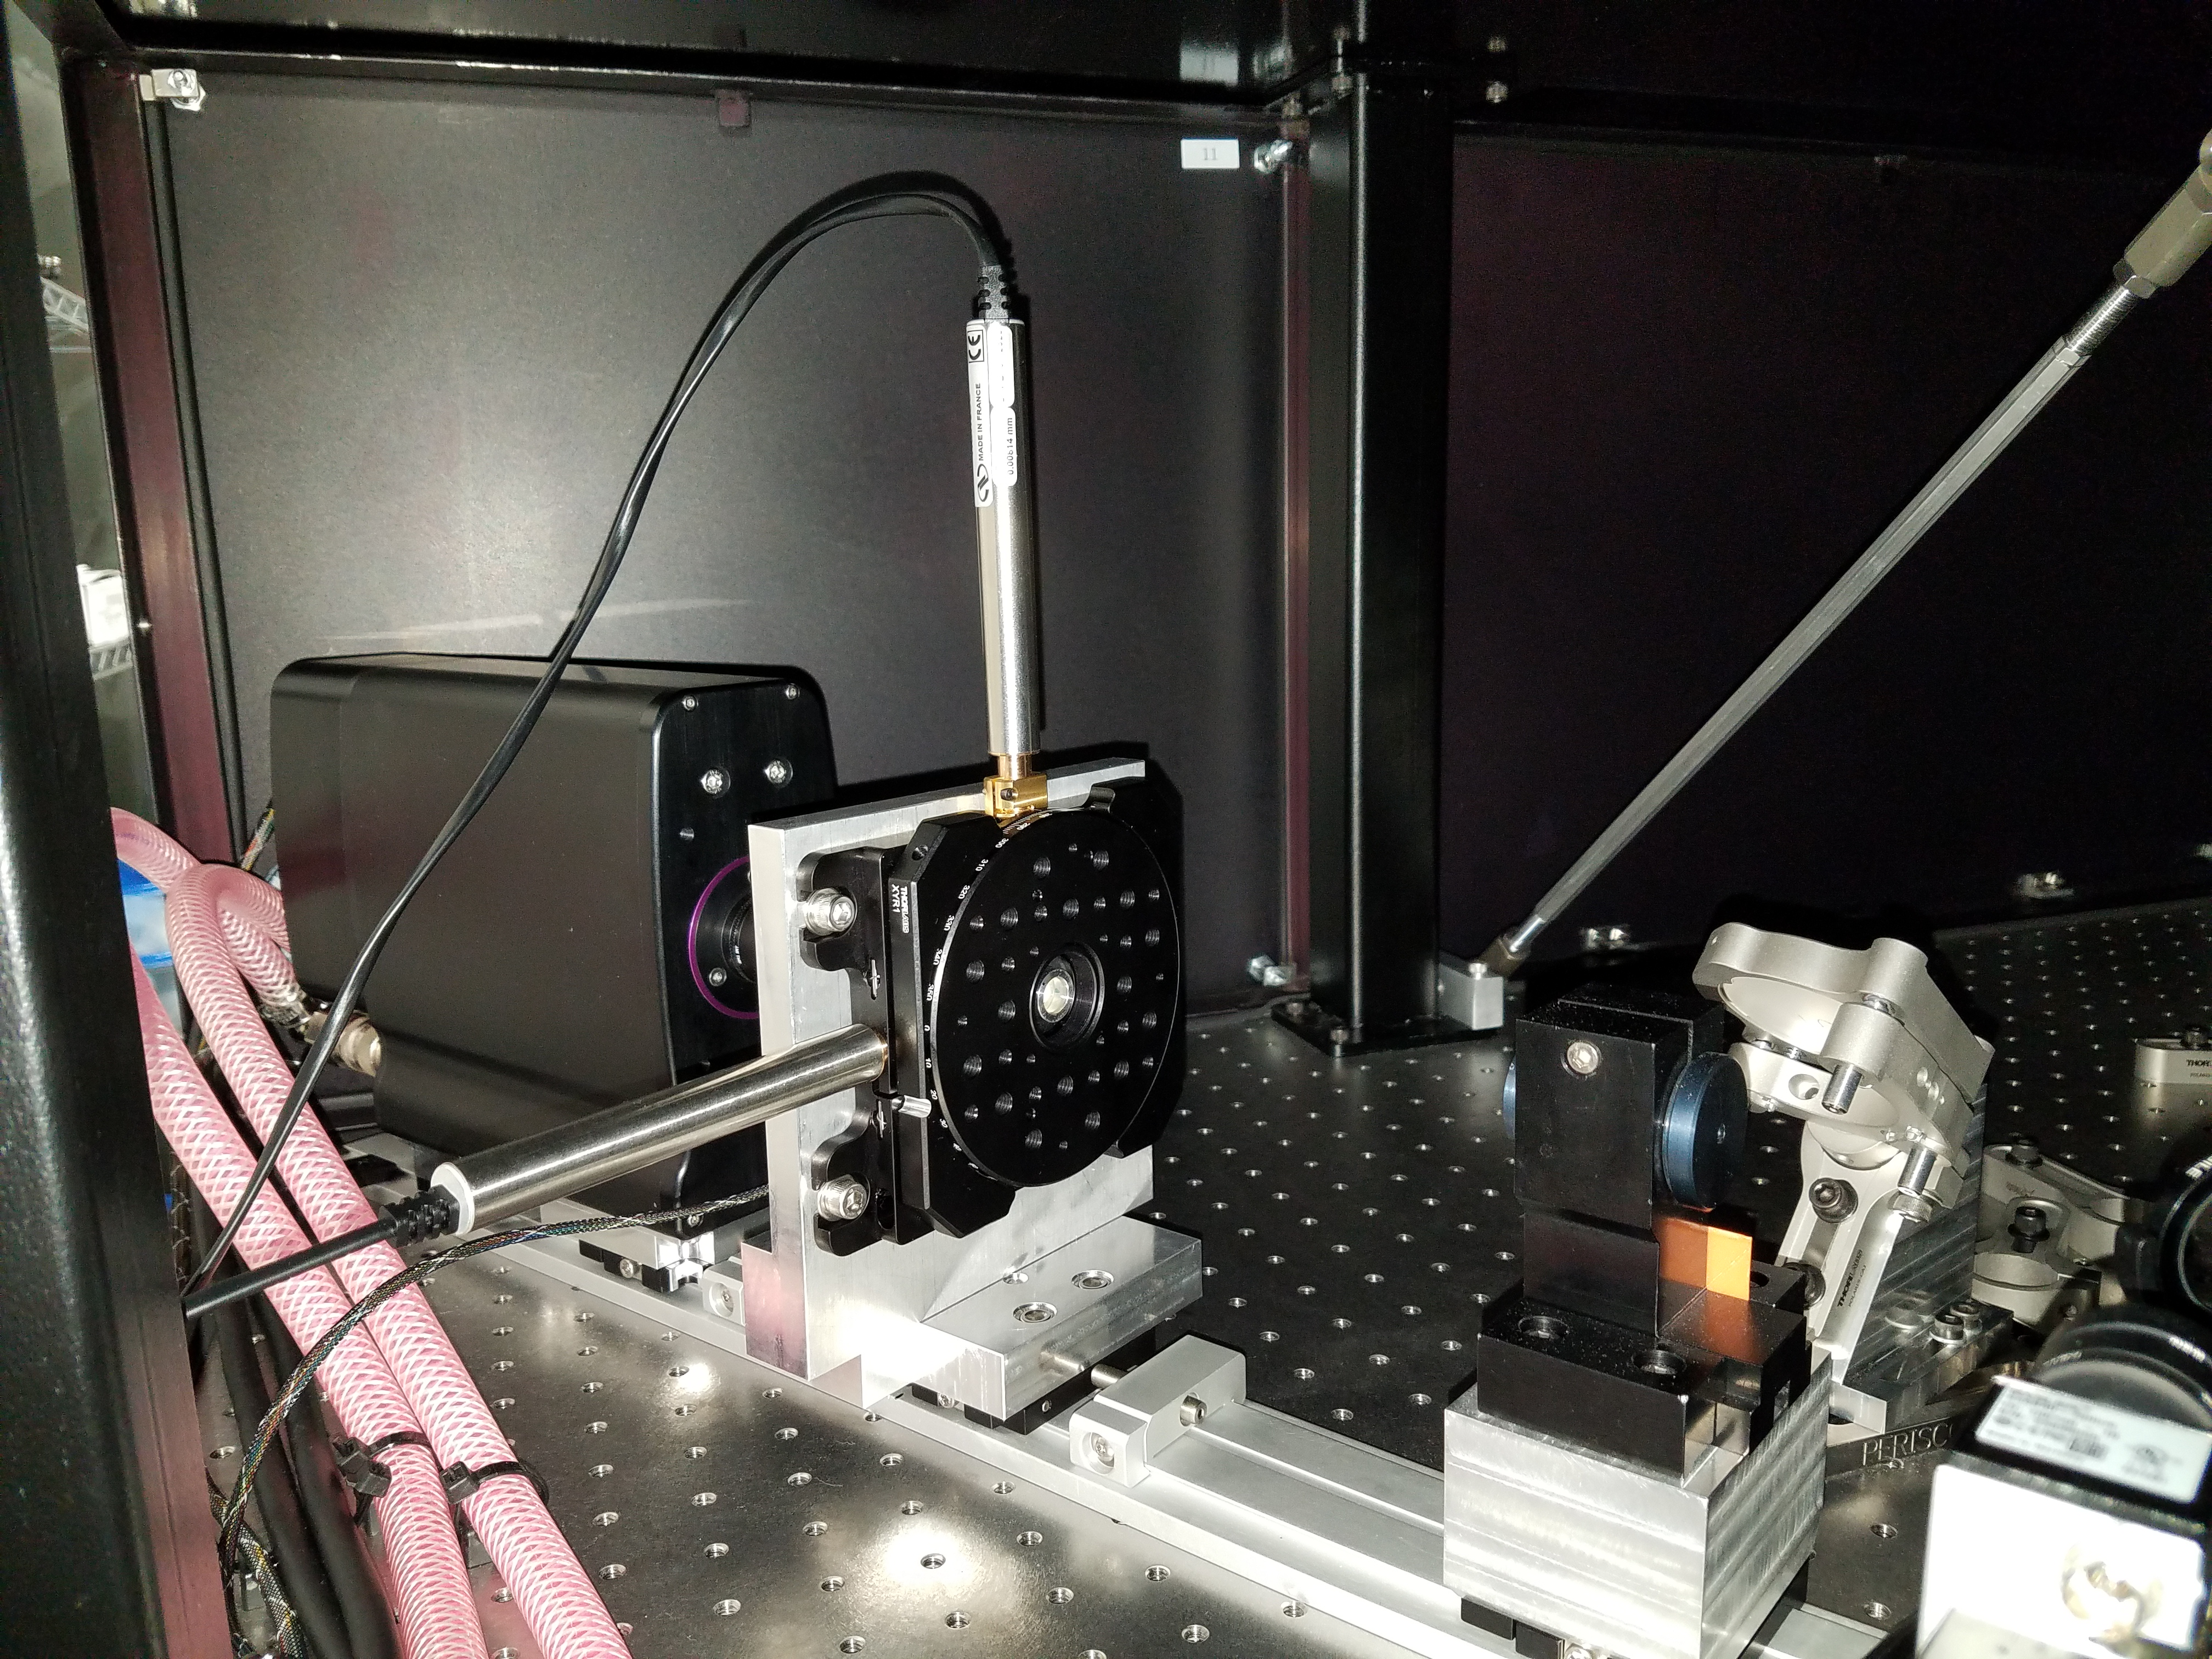
\includegraphics[width=.8\textwidth]{Chapter Materials/Chapter Three Materials/cameraLensPiezoHolder.png}
    \caption{The custom achromatic triplet lens mounted in a precision X-Y lens mount.}
    \label{fig:mountedtriplet}
\end{figure}
	
An initial alignment of the MagAO-X pyramid wavefront sensor was done using a HeNe single mode fiber laser, two off axis parabolic mirrors, and a temporary pupil mask with coarse edges. The pyramid optic, camera lens, and OCAM$^2$K were mounted on a coaxial rail system from ThorLabs as shown in Figure \ref{fig:mountedPWFS}. Custom mounting plates were fabricated for each optic, so that each could be mounted onto rail carriages and meet the beam height requirement of 5 inches from the optical table. 

\begin{figure}
    \centering
    \includegraphics[width=.8\textwidth]{Chapter Materials/Chapter Three Materials/mountedPWFS.jpg}
    \caption{The mounted pyramid optics, camera lens, and OCAM$^2$K camera on a coaxial rail from ThorLabs.}
    \label{fig:mountedPWFS}
\end{figure}

The mount of the pyramid optic has a custom target that aligns with the pyramid tip. To align the PWFS we first mounted the pyramid optic with the target on the optical rail and placed it on the MagAO-X optical table. The position of the rail and the tip/tilt of the incoming beam from OAP $\#5$, was adjusted iteratively until the beam hit the center of the target when the pyramid was placed at both the front and the back of the rail. This established the beam line for the system. The camera lens and OCAM$^2$K was then placed on the rail according to the Zemax design. The fine focus of the pyramid optic was dialed using a micrometer nudger, and by examining the signal of the pyramid pupils with and without modulation. The spacing of the camera lens and the OCAM$^2$ were adjusted until the size and separation of the pupils were in specifications. The measurement of the pupil parameters was done by a circle fit of the modulated pyramid pupils shown in Figure \ref{fig:fitPupils}. The average size of the MagAO-X pupils is 55.83 pixels in diameter. Figure \ref{fig:MagAOXpupils} shows the white light pupils of the MagAO-X PWFS under 5 $lambda/D$ modulation.

\begin{figure}
    \centering
    \includegraphics[width=.8\textwidth]{Chapter Materials/Chapter Three Materials/Age 170.668.jpeg}
    \caption{Caption}
    \label{fig:fitPupils}
\end{figure}

\begin{figure}
    \centering
    \includegraphics{Chapter Materials/Chapter Three Materials/MagAOXpupil5LD.png}
    \caption{The MagAO-X pyramid wavefront sensor pupils with 5 $\lambda/D$ modulation. The spiders and central obscuration are from the aperture of the Magellan Telescope.  }
    \label{fig:MagAOXpupils}
\end{figure}
\chapter{Simulations and Analysis of the 3PWFS}

To assess the performance of the 3PWFS compared to the 4PWFS, a simulation was developed using the Object Oriented Matlab Adaptive Optics toolbox (OOMAO) \cite{OOMAO}. The OOMAO toolbox is an end-to-end adaptive optics model that can simulate different combinations of guide stars, turbulent atmospheres, wavefront sensors, deformable mirrors, and science cameras. Light is propagated using Fraunhofer diffraction. The master OOMAO toolbox simulates a 4PWFS using Slopes Maps. This chapter details the work that was done to extend OOMAO's ulitilies to include the 3PWFS and the Raw Intensity signal processing method. We then detail an experiment performed on OOMAO to study the performance of the 3PWFS compared to the 4PWFS for different magnitude guide stars. 

\section{The Object Oriented Matlab Adaptive Optics toolbox}

The OOMAO toolbox is a library of classes that are used to assemble objects that simulate different components of an adaptive optics system. The electric field is propagated object to object according to the optical path of a real AO system. The main classes include: The source class, atmosphere telescope class, deformable mirror class, pyramid class, and the detector class. The source class generates the beacon guide star used by the AO system for wavefront sensing. The guide star object contains the information of the wavelength bandpass of the system, and the user can set the magnitude of the guide star to change the intensity of light at the detector. The light from the guide star is propagated through the atmosphere to the telescope object. The atmosphere class generates the phase screens that are used to simulate turbulence. The number of layers, the wind speed, Fried parameter $r_0$, and outer and inner scale of the turbulence profile can be set. The resulting phase screens are scaled and compressed into a single phase screen in the pupil plane.  The telescope object defines the aperture of the system, the system resolution, and the exposure time. The default setting is a clear circular aperture, but central obscurations can be modeled from within OOMAO. The user can provide their own pupil mask for more complex apertures. The deformable mirror object contains the basis set used for modal wavefront sensing. In the OOMAO library there are class files to generate Zernike modes and Fourier modes. The number of actuators and the influence function of each actuator can be set by the user. For our simulations we use a Bezier influence function which is one of the provided influence functions by OOMAO. The pyramid object simulates the pyramid wavefront sensor by using a phase mask to simulate the pyramid tip. The user can select the number of facets, and the apex angle of the pyramid which sets the separation on the WFS detector. The sampling of each of the pupils and the radius of modulation are also user defined attributes to this object. The detector object records the intensity at the focal plane. At the detector the user can turn on photon noise, as well as set the read noise for the detector. 

\begin{lstlisting}[language=Python, caption=Python example]
ngs=source
\end{lstlisting}







\section{The Pyramid Object}
\subsection{The Phase Screen}
\subsection{Signal Handling}
\subsection{Calibration}





The PWFS is simulated using a single tip/tilt phase mask that is segmented into N parts. Figure \ref{fig:oomaoFigs}.A and \ref{fig:oomaoFigs}.C show the masks for the 3PWFS and 4PWFS. The masks are scaled and rotated according to a user input for rotation and pyramid apex angle that controls the separation of the pyramid pupils. After scaling, the mask is converted into a phase mask that is applied at the focal plane to simulate a pyramid tip. Figure \ref{fig:oomaoFigs}.C and \ref{fig:oomaoFigs}.D show the resulting pyramid pupils on the simulated wavefront sensor camera, using a flat wavefront and 5 $\lambda/D$ modulation. The master OOMAO toolbox simulates a 4PWFS using Slopes Maps. We extended the PWFS class in OOMAO to include a 3PWFS, taking care that the amplitude of the tip/tilt phase in the 3PWFS phase screen generation matched that of 4PWFS. We included our derivation of the Slopes Maps equation for the 3PWFS (derived in Section~\ref{SlopesDerivation} below), and added the Raw Intensity method for both the 4PWFS and the 3PWFS. For both the Slopes Maps and Raw Intensity method the signal was normalized by the mean value across all valid pixels on the wavefront sensor detector, instead of normalizing pixel by pixel. 

\begin{figure}
    \centering
    \includegraphics[width=1\textwidth]{oomaoFigs.png}
    \caption{Details of the simulated PWFS in OOMAO. A) and B) The simulated 3PWFS and 4PWFS pyramid masks in OOMAO. These masks are used as a phase screen in the pupil plane to emulate the focal plane splitting and separation done by a real glass pyramid. C) and D) The pupils from the 3PWFS and 4PWFS respectively on the simulated detector. In OOMAO the user can change the size, separation, and intensity values of the pupils through user defined inputs.}
    \label{fig:oomaoFigs}
\end{figure}


\section{Performance Comparison of the 3PWFS and 4PWFS}
\subsection{Simulation}

Using OOMAO an end to end simulation of an adaptive optics system was written to compare the performance of the 3PWFS and 4PWFS using both Raw Intensity and Slopes.  The goal was to measure the quality of correction from the AO closed loop by calculating the Strehl Ratio produced by each wavefront sensor as a function of guide star magnitude. In this simulation the Strehl ratio was calculated using OOMAO's built in Strehl calculator, which uses the OTF calculated from a PSF with no phase aberration, and a PSF with AO compensated phase aberration. The details of the simulation are summarized in the flow chart in Figure \ref{fig:simulationl}. To characterize the sensitivity of each sensor to read noise the following experiment was performed twice, once at $0.5e^-$ read noise to match that of an OCAM2K camera, and once at $12 e^-$ read noise to match the noisest camera on the Comprehensive Adaptive Optics and Coronagraph Test Instrument (CACTI) at the UA Extreme Wavefront Control Lab (XWCL). Listed below is the experiment performed in OOMAO:

\begin{itemize}
    \item Guide star magnitude was varied incrementally from 0 to 12th magnitude in steps of 2.
    \item At each magnitude closed loop data was taken with different loop gains from 0.1 to 1.8 in steps of 0.1.
    \item At each loop gain the performance was tested by closing the loop on 15 different atmospheric realizations and recording 500 closed loop PSF frames. 
    \item Strehl values were calculated from the PSFs and an average Strehl ratio is reported for a given loop gain at a given magnitude.
    \item The loop gain that gave the highest Strehl value for that guide star magnitude was used in the final calculation of Strehl vs guide star magnitude.
    \item The result is a plot of Strehl versus guide star magnitude, where the value of Strehl has been optimized over the loop gain shown in Figure \ref{fig:overall}
\end{itemize}


\begin{figure}
    \centering
    \includegraphics[width=0.8\textwidth]{simulation.png}
    \caption{Experimental details of the simulation done in OOMAO. Light starts at the natural guide star and is propagated through the atmosphere, telescope and wavefront sensor. The wavefront sensor measures a correction that is then applied by the deformable mirror.  The resulting AO corrected PSF is recorded on a noiseless science camera. }
    \label{fig:simulationl}
\end{figure}

\subsection{Results}

In Figure \ref{fig:overall}, no significant difference in performance was found in the comparison case of the wavefront sensors with 0.5$e^-$ read noise. Most on-sky adaptive optics systems use a 4PWFS with Slopes (4PWFS SM) so we use this wavefront sensor as our reference for comparison. The performance of each wavefront sensor was found to be within a percent of Strehl from the 4PWFS SM, across all stellar magnitudes. For the simulations at 12$e^-$ read noise in Figure \ref{fig:overall} a gain of 0.0359 Strehl was found for the 3PWFS using Raw Intensity (3PWFS RI) over the 4PWFS SM at a stellar magnitude of 10. At the same magnitude the 4PWFS RI also out performed the 4PWFS SM, but the gain was only 0.0122 Strehl. This simulation successfully showed the gain in performance from the 3PWFS at low light levels where the effects of read noise are stronger. The overall performance of each wavefront sensor at each guide star magnitude is given in Figure \ref{fig:overall}. In Figures \ref{fig:0RN} and \ref{fig:12RN} comparison plots were made by subtracting the Strehl values for 4PWFS SM from the other wavefront sensors, to help visualize the performance of each wavefront sensor. From these results we can conclude that the 3PWFS is a viable wavefront sensor with performance comparable to a 4PWFS.


\begin{figure}[h]
    \centering
    \includegraphics[width=0.8\textwidth]{StrehlvGuideStar4v3.png}
    \caption{Strehl vs Guide Star magnitude for each PWFS. The steep drop off in performance of the lower curves is due to the effects of 12$e^-$ read noise. At guide star magnitude of 10, the read noise starts to matter, and the 3PWFS out performs the 4PWFS. }
    \label{fig:overall}
\end{figure}


\begin{figure}[h]
    \centering
    \includegraphics[width=.7\linewidth]{StrehlvGuideStarvs4PWFSRM0e.png}
    \caption{Comparison plot of wavefront sensor performance vs the 4PWFS using Slopes at 0.5 $e^-$ read noise. }
    \label{fig:0RN}
\end{figure}

\begin{figure}[h]
    \centering
    \includegraphics[width=.7\linewidth]{StrehlvGuideStarvs4PWFSRM12e.png}
    \caption{Comparison plot of wavefront sensor performance vs the 4PWFS using Slopes at 12 $e^-$ read noise.}
    \label{fig:12RN}
\end{figure}

\newpage
\chapter{Simulations and Analysis of the 3PWFS}\label{CH4}

To assess the performance of the 3PWFS compared to the 4PWFS, a simulation was developed using the Object Oriented Matlab Adaptive Optics toolbox (OOMAO) \citep{OOMAO}. The OOMAO toolbox is an end-to-end adaptive optics model that can simulate different combinations of guide stars, turbulent atmospheres, wavefront sensors, deformable mirrors, and science cameras. Light is propagated using Fraunhofer diffraction. The master OOMAO toolbox simulates a 4PWFS using Slopes Maps. This chapter details the work that was done to extend OOMAO's utilities to include the 3PWFS and the Raw Intensity signal processing method. We then discuss an experiment performed in OOMAO to study the performance of the 3PWFS compared to the 4PWFS for different magnitude guide stars.

In Section \ref{WFSerror} the SNR for the 3PWFS and 4PWFS was calculated for varying guide star magnitudes. At low light levels when the read noise term dominates the 3PWFS has a gain of $\sqrt{4/3}$ in SNR over the 4PWFS. Other benefits of using a 3PWFS is the simplified manufacturing process. Grinding and polishing a high quality three-sided pyramid optic is faster and cheaper than a four-sided pyramid optic of similar quality. A concern for the 3PWFS is that the wavefront is sampled with three points instead of four. The 3PWFS potential has a larger null space than the 4PWFS, meaning less modes are sensed and the accuracy of the wavefront sensing is reduced. In this and the following chapter we characterize the performance of the 3PWFS in both simulation and on a testbench to explore the potential benefits and disadvantages of the 3PWFS.


\section{The Object Oriented Matlab Adaptive Optics toolbox}

The OOMAO toolbox is a library of classes that are used to assemble objects that simulate different components of an adaptive optics system. The electric field is propagated object to object according to the optical path of the simulated AO system. The main classes include: The source class, atmosphere telescope class, deformable mirror class, pyramid class, and the detector class. The source class generates the beacon guide star used by the AO system for wavefront sensing. The guide star object contains the information of the wavelength bandpass of the system, and the user can set the magnitude of the guide star to change the intensity of light at the detector. The light from the guide star is propagated through the atmosphere to the telescope object. The atmosphere class generates the phase masks that are used to simulate turbulence. The number of layers, the wind speed, Fried parameter $r_0$, and outer and inner scale of the turbulence profile can be set. The resulting phase masks are scaled and compressed into a single phase mask in the pupil plane.  The telescope object defines the aperture of the system, the system resolution, and the exposure time. The default setting is a clear circular aperture, but central obscurations can be modeled from within OOMAO. The user can provide a pupil mask for more complex apertures. The deformable mirror object contains the basis set used for modal wavefront sensing. In the OOMAO library, there are class files to generate Zernike modes and Fourier modes. The number of actuators and the influence function of each actuator can be set by the user. For our simulations, we use a Bezier influence function which is one of the provided influence functions by OOMAO. The pyramid object uses a phase mask to simulate the pyramid tip. The user can select the number of facets, and the apex angle of the pyramid which sets the separation on the WFS detector. The sampling of each of the pupils and the radius of modulation are also user-defined attributes to this object. The detector object records the intensity at the focal plane. At the detector, the user can turn on photon noise, as well as set the read noise for the detector. 

% Listed below is example code to generate the objects in OOMAO.

% \begin{lstlisting}[language=Matlab]
% %% Guide Star
% % Single guide star at infinity, R-band wavelength.
%     ngs=source('wavelength',photometry.R);

% % Science source for Strehl calculation
%     science=source('wavelength',photometry.R);

% %% Atmosphere
% %Fried parameter [m]
%     r0=16e-2;
% %Outer Scale [m]
%     L0=6.25; 
% %Wind speed [m/s]
%     v=7.4;      

% % makes an atmosphere object with the given parameters 
% %at the given wavelength
%     atm=atmosphere(photometry.R,r0,L0,'windSpeed',...
%     v,'windDirection',0);

% %% Telescope
% %Diameter of the telescope in meters
%     D=2  
% %Diameter of the circular entrance pupil in pixels.
% %Sets the sampling of the phase that is generated.
% %Adjust to avoid alaising.
%     nPx=240     
             
% %Frequency in Hz. Sets the integration time and 
% %the simulated loop speed.
%     freq=300    
            

%     tel= telescope(D,'resolution',nPx,...
%     'samplingTime',1/freq);

% %% Deformable Mirror
% %Generates a deformable mirror, that is a grid of actuators 
% %that fill a circular aperture

% %Diameter in actuators of the circular aperture of the DM
%     nAct=9;   
% %Max spatial frequency corrected by the DM
%     d=D/(nAct-1);
%     fmax=1/(2*d); 
% %Max mode # corrected by the DM
%     nMax=ceil(D*fmax/0.37-1);       



% %Zernike basis set
% %Number of modes in the basis set to generate
%     nModes=sum(1:nMax+1)-1;         
% %Zernike basis set generation
% %zern=zernike(2:nModes+1, D, 'resolution', nPx);  
% %Bezier Influence function
%     bif = influenceFunction('monotonic',30/100);    
% %Generates the circular aperture of the DM
%     v=utilities.circle(nAct,nAct);  

% % Deformable mirror object
%     dm = deformableMirror(nAct,...
%         'modes',bif,...
%         'resolution',nPx,...
%         'validActuator',logical(v));

% %% Wavefront Sensor
% %PWFS pupils 20 pixels in diameter
%     nSamp=20 
% %Modulation radius 5 lambda/D
%     mod=5
% %Apex angle of the pyramid. 
% %Sets the separation of pupils
%     alpha=pi/3 
% %Number of sides on the pyramid. 
% %3 and 4 used for simulation.
%     nFaces=3        

% %ngs = guide star object
% %tel= telescope object
% %FWHM in pixels of the focal point spot on the pyramid tip
%     c=2
% %Rotates the pyramid mask to change 
% %orientation of pupils on the detector
%     rotation=3*pi/2

% %Flag that controls what PWFS signal handling method is used. 
% %0 is Slopes Maps, 2 is Raw Intensity. 
% %1 was a failed experiment ignore.
%     altSlopes=0            
% %A flag used to generate an alternative 
% %phase mask for the 3PWFS tip
% %For use on the Spatial Light Modulator on LOOPs. Ignore.                        
%     alternative=0                                       
                        
%     wfs = pyramid(nSamp,nPx,'modulation',mod, 
%     'alpha',alpha,'nFaces',nFaces, 'src',ngs,...
%     'tel',tel, 'c', c,'rotation',rotation,...
%     'altSlopes',altSlopes,... 
%     'alternative', alternative);

% %% Science Camera
% %generates the science camera object with a focal plane 
% %resolution given by the diameter of the telescope aperture.

%     cam=imager('diameter', tel.D);
% \end{lstlisting}



\section{The Pyramid Class}
The master OOMAO toolbox simulates a 4PWFS using Slopes Maps. This section details the changes made to the pyramid class to simulate the 3PWFS. Appendix \label{OOMAOcode} lists the code that is discussed in this section. 


\subsection{The Pyramid Phase mask}
The PWFS is simulated using a single tip/tilt phase mask that is segmented into N parts. The mask is applied in the focal plane to simulate the pyramid tip. In the master OOMAO toolbox, the function that generated the pyramid tip phase mask only generated a 4PWFS mask. To generate the 3PWFS mask, code was adapted from the function that generated the phase masks for the spatial light modulator on the LOOPs testbed. The code was adjusted to have the same scaling as the original mask generator so that a given apex angle gives the same pupil separation for both functions.
\begin{figure}
    \centering
    \includegraphics[width=1\textwidth]{Chapter Materials/Chapter Four Materials/phaseMask.png}
    \caption{A. The spiral grid of angular values used to determine where to segments the PWFS facets based on rotation and number of facets. B.C.D. Examples of the binary masks used to segment the pupil plane. Each mask is then given a tip/tilt phase and summed to create the phase mask that simulates the pyramid tip. }
    \label{fig:phaseMask}
\end{figure}

 The mask function works to creates a spiral grid of angular values from $-\pi$ to $\pi$ starting in the center of the frame, as shown in Figure \ref{fig:phaseMask}.A. The grid is used to segment the focal plane corresponding to the number and the rotation of the facets. A mask is made for each facet; and an example of the 3PWFS facet masks are shown in Figure \ref{fig:phaseMask}.B, Figure \ref{fig:phaseMask}.C, and Figure \ref{fig:phaseMask}.D. A tip/tilt phase is added to each of the facet masks and then scaled according to a user inputted apex angle. The masks are then summed to produce the final phase mask for the pyramid tip. Figure \ref{fig:oomaoFigs}.A and \ref{fig:oomaoFigs}.C show the masks for the 3PWFS and 4PWFS. Figure \ref{fig:oomaoFigs}.C and \ref{fig:oomaoFigs}.D shows the resulting pyramid pupils on the simulated wavefront sensor camera, using a flat wavefront and 5 $\lambda/D$ modulation. 

\begin{figure}
    \centering
    \includegraphics[width=1\textwidth]{Chapter Materials/Chapter Four Materials/oomaoFigs.png}
    \caption{Details of the simulated PWFS in OOMAO. A) and B) The simulated 3PWFS and 4PWFS pyramid masks in OOMAO. These masks are used as a phase mask in the pupil plane to emulate the focal plane splitting and separation done by a real glass pyramid. C) and D) The pupils from the 3PWFS and 4PWFS respectively on the simulated detector. In OOMAO the user can change the size, separation, and intensity values of the pupils through user defined inputs.}
    \label{fig:oomaoFigs}
\end{figure}

\subsection{Signal Handling}

The master OOMAO toolbox simulates a 4PWFS using Slopes Maps. We extended the PWFS class in OOMAO to include the Slopes Maps equations for both the 3PWFS and the 4PWFS, as well as the Raw Intensity method. The pyramid class in OOMAO was hard-coded to expect a matrix size that corresponded to the Slopes Maps signals. For example if the pupils are 20 pixels in diameter, the SM measurement would be a 20x40 matrix, because it produces both a $S_x$ and a $S_y$ measurement. The Raw Intensity signal is a matrix the size of the full frame of the detector. Part of this work was to restructure the pyramid class to accept an arbitrary matrix size.  We included our derivation of the Slopes Maps equation for the 3PWFS derived in Section \ref{Slopes}. For both the Slopes Maps and Raw Intensity method the signal was normalized by the mean value across all valid pixels on the wavefront sensor detector, instead of normalizing pixel by pixel. 

The Slopes Maps calculation requires the knowledge of the location of the pupils on the detector. Each pupil is cropped out and combined with the other pupils for the SM calculation. In the master OOMAO class, the location of the pupil is determined by a calibration step that generates a PWFS with high modulation and a propagated wavefront that contains no phase error. The result is highly uniform pupils on the detector. The detector is split into four quadrants, and each quadrant is thresholded to create a valid detector pixel mask. In the SM calculation, the PWFS signal is divided the same way, and the valid detector pixel mask for each quadrant is applied. This methodology is incompatible with the new way of generating the PWFS masks, which allows for an N-sided pyramid with rotation. A new method of determining the valid detector pixels was developed to be more robust for different PWFS. This method uses the same calibration PWFS. The detector image is thresholded to mask out any pixels with a low signal. The thresholded image is then converted into a binary mask, where the pixels that contain the pupil signals have a value of 1, and all other pixels have a value of 0. Built-in Matlab functions are then used to detect regions, and calculate the centroid of those regions. The resulting binary masks for the 3PWFS and 4PWFS are shown in Figure \ref{fig:pyrcen} A and B. Over-plotted is the location of the calculated centroid given by a dot in the center of each of the regions. OOMAO uses the centroid coordinates to pull out each of the pupils for the SM calculation.

\begin{figure}
    \centering
    \includegraphics[width=.8\textwidth]{Chapter Materials/Chapter Four Materials/pyramidCenters.png}
    \caption{The calculated binary masks used to detect the location of the pyramid pupils. Over-plotted is the location of the calculated centroid given by a dot in the center of each of the regions.}
    \label{fig:pyrcen}
\end{figure}


\section{Performance Comparison of the 3PWFS and 4PWFS}
\subsection{Simulation}

Using OOMAO an end-to-end simulation of an adaptive optics system was written to compare the performance of the 3PWFS and 4PWFS using both Raw Intensity and Slopes.  The goal was to measure the quality of correction from the AO closed loop by calculating the Strehl Ratio produced by each wavefront sensor as a function of guide star magnitude. In this simulation, the Strehl ratio was calculated using OOMAO's built-in Strehl calculator, which uses the OTF calculated from a PSF with no phase aberration, and a PSF with AO compensated phase aberration. The details of the simulation are summarized in the flow chart in Figure \ref{fig:simulationl}. To characterize the sensitivity of each sensor to read noise the following experiment was performed twice, once at $0.5e^-$ read noise to match that of an OCAM2K camera, and once at $12 e^-$ read noise to match the noisest camera on the Comprehensive Adaptive Optics and Coronagraph Test Instrument (CACTI) at the UA Extreme Wavefront Control Lab (XWCL). Listed below is the experiment performed in OOMAO:

\begin{itemize}
    \item Guide star magnitude was varied incrementally from 0 to 12th magnitude in steps of 2.
    \item At each magnitude closed loop data was taken with different loop gains from 0.1 to 1.8 in steps of 0.1.
    \item At each loop gain the performance was tested by closing the loop on 15 different atmospheric realizations and recording 500 closed loop PSF frames. 
    \item Strehl values were calculated from the PSFs and an average Strehl ratio is reported for a given loop gain at a given magnitude.
    \item The loop gain that gave the highest Strehl value for that guide star magnitude was used in the final calculation of Strehl vs guide star magnitude.
    \item The result is a plot of Strehl versus guide star magnitude, where the value of Strehl has been optimized over the loop gain shown in Figure \ref{fig:overall}
\end{itemize}


\begin{figure}
    \centering
    \includegraphics[width=0.8\textwidth]{Chapter Materials/Chapter Four Materials/simulation.png}
    \caption{Experimental details of the simulation done in OOMAO. Light starts at the natural guide star and is propagated through the atmosphere, telescope and wavefront sensor. The wavefront sensor measures a correction that is then applied by the deformable mirror.  The resulting AO corrected PSF is recorded on a noiseless science camera. }
    \label{fig:simulationl}
\end{figure}

\subsection{Results}

In Figure \ref{fig:overall}, no significant difference in performance was found in the comparison case of the wavefront sensors with 0.5$e^-$ read noise. Most on-sky adaptive optics systems use a 4PWFS with Slopes (4PWFS SM) so we use this wavefront sensor as our reference for comparison. The performance of each wavefront sensor was found to be within a percent of Strehl from the 4PWFS SM, across all stellar magnitudes. For the simulations at 12$e^-$ read noise in Figure \ref{fig:overall} a gain of 0.036 Strehl was found for the 3PWFS using Raw Intensity (3PWFS RI) over the 4PWFS SM at a stellar magnitude of 10. At the same magnitude, the 4PWFS RI also outperformed the 4PWFS SM, but the gain was only 0.012 Strehl. This simulation successfully showed the gain in performance from the 3PWFS at low light levels where the effects of read noise are stronger. The overall performance of each wavefront sensor at each guide star magnitude is given in Figure \ref{fig:overall}. In Figures \ref{fig:0RN} and \ref{fig:12RN} comparison plots were made by subtracting the Strehl values for 4PWFS SM from the other wavefront sensors, to help visualize the performance of each wavefront sensor. From these results, we can conclude that the 3PWFS is a viable wavefront sensor with performance comparable to a 4PWFS.


\begin{figure}[h]
    \centering
    \includegraphics[width=0.8\textwidth]{Chapter Materials/Chapter Four Materials/StrehlvGuideStar4v3.png}
    \caption{Strehl vs Guide Star magnitude for each PWFS. The steep drop off in performance of the lower curves is due to the effects of 12$e^-$ read noise. At guide star magnitude of 10, the read noise starts to matter, and the 3PWFS out performs the 4PWFS. }
    \label{fig:overall}
\end{figure}


\begin{figure}[h]
    \centering
    \includegraphics[width=.7\linewidth]{Chapter Materials/Chapter Four Materials/StrehlvGuideStarvs4PWFSRM0e.png}
    \caption{Comparison plot of wavefront sensor performance vs the 4PWFS using Slopes at 0.5 $e^-$ read noise. }
    \label{fig:0RN}
\end{figure}

\begin{figure}[h]
    \centering
    \includegraphics[width=.7\linewidth]{Chapter Materials/Chapter Four Materials/StrehlvGuideStarvs4PWFSRM12e.png}
    \caption{Comparison plot of wavefront sensor performance vs the 4PWFS using Slopes at 12 $e^-$ read noise.}
    \label{fig:12RN}
\end{figure}

\subsection{Discussion}


\cite{codona2018comparative} used the AOsim3 wave optics package to compare end to end performance of a 3PWFS to a 4PWFS with no modulation. In this simulation the Raw Intensity  signal handling method was used. In open loop with no noise the study showed that the 4PWFS out performed the 3PWFS by 0.005 Strehl. Our simulation results agree with the findings by Codona et al. We found in our simulations with 0.5 read noise that the performance of the wavefront sensors are within 0.01 Strehl. Our results differ from Codona et al. when including read noise. They found that for a detector with $3e^-$ read noise, that there was a gap performance improvement by 1 guide star magnitude in favor of the 3PWFS. Codona et. al. considered other factors including system latency, and were sensing in the visible. Our simulations are in r-band and were optimized only for loop gain. Using a detector with $12 e^-$ read noise we found that the performance of the wavefront sensors are once again comparable, and we found only $~0.02$ gain in Strehl from the 3PWFS at 10th magnitude. The scope of our simulations is limited but still agree that the 3PWFS is less sensitive to read noise, however the amount of improvement gained is still under question. Both the 3PWFS and 4PWFS discussed in this paper are refractive, and image all pupils onto the same detector \citep{sanchez2020design}. Moving towards a reflective PWFS that would image each pupil onto its own detector could have a more substantial benefit. Each detector would be smaller, resulting in faster readout speeds with less added read noise. Low read noise detectors are expensive, so using a reflective PWFS would increase system cost and complexity.

\newpage
\chapter{Experimental Demonstration of the Three-Sided Pyramid Wavefront Sensor on the CACTI Testbed}\label{CH6}

The next generation of giant ground and space telescopes will have the light-collecting power to detect and characterize potentially habitable terrestrial exoplanets for the first time. This will only be achievable if the performance of GSMT-ExAO systems is optimized. The ground based GSMTs include the Thirty Meter Telescope (TMT) \citep{chisholm2020thirty}, the Giant Magellan Telescope (GMT) \citep{fanson2020overview}, and the European Extremely Large Telescope (E-ELT) \citep{ramsay2020eso}. Various testbeds are advancing technology and techniques to enable exoplanet imaging on the next generation of telescopes. Current testbeds include the High Contrast Imager for Complex Aperture Telescopes (HiCAT) \citep{2014SPIE.9143E..27N}, at the Space Telescope Science Institute, the Decadal Survey Testbed \citep{ruane2019decadal}, at the NASA Jet Propulsion Laboratory (JPL), LAM-ONERA On-sky Pyramid Sensor (LOOPS) \citep{janin2019adaptive}, at the Laboratoire d'Astrophysique de Marseille, and the High Contrast High- Resolution Spectroscopy for Segmented telescopes testbed (HCST) \citep{jovanovic2018high}, at the California Institute of Technology. The Magellan Extreme Adaptive Optics system (MagAO-X) \citep{males2020magao}, developed for the Magellan Clay Telescope, doubles as an ExAO testbed. The Subaru Coronagraphic Extreme Adaptive Optics instrument (SCExAO) \citep{jovanovic2015subaru}, is similarly used to advance ExAO technology. There are many more high-contrast imaging testbeds in existence, and many are listed on the Community of Adaptive Optics and High Contrast testbeds website \citep{CHAOTIC}. A recent summary of current coronagraphy testbeds for space missions can be found in the decadal white paper by \cite{mazoyer2019high}.

Here we present the Comprehensive Adaptive Optics and Coronagraph Test Instrument (CACTI), which was designed with the flexibility to support visiting instruments and to be easily re-configurable to perform multiple experiments.  We first describe the design of CACTI, review its operation and calibration procedures, and discuss its current status. We then discuss an experiment performed on CACTI with a visiting three-sided pyramid wavefront sensor (3PWFS) to explore an alternative wavefront sensor architecture for GSMT-ExAO. Both a 3PWFS and 4PWFS were integrated into  CACTI to demonstrate the operation of a 3PWFS and compare it to the 4PWFS. We present results from experiments demonstrating the operation of the 3PWFS, and comparisons to the 4PWFS. Finally, we discuss the outcome of these experiments.

\section{Design of CACTI}
CACTI was designed to model a full end-to-end adaptive optics system with the flexibility to support multiple experiments. In the configuration described here, CACTI consisted of two components: an adaptive optics simulator and a pyramid wavefront sensor testbed. In the following sections, we describe the optical design in detail. 

\subsection{Adaptive Optics Simulator}

\begin{figure}
    \centering
    \includegraphics[width=0.8\textwidth]{Chapter Materials/Chapter Five Materials/CACTIzemax.png}
    \caption{Optical design of CACTI. Light starts from a point source from the HeNe laser and relayed through a series of afocal pupil relays. The focal plane of the AO simulator is after the 6${^{th}}$ OAP. It is collimated by a lens and passed into the PWFS testbed. A beamsplitter sends the same focal plane to both the 3PWFS and 4PWFS to minimize non-common path errors.}
    \label{fig:CACTIZemax}
\end{figure}

CACTI was designed to simulate atmospheric turbulence in a complete closed loop AO system. The optical design of  CACTI  is shown in Figure \ref{fig:CACTIZemax} and Table \ref{tab:CACTItable} summarizes the main components. The layout on the optical table is shown in Figure \ref{fig:CACTI}. A Helium-Neon (HeNe) laser (wavelength 633-$nm$) is used for inital alignment and testing.  The light is passed to a spatial filter with a 10-$\mu m$ pinhole to clean up any wavefront errors, and insure that the start of the system is an unresolved point source. The point source is then collimated by an off-axis parabolic (OAP) mirror to simulate starlight coming from infinity. There are six OAP mirrors in total that form the pupil relays of the system. All are cored from the same parent with $\lambda /10$ surface quality (Peak-to-Valley). Each OAP has a focal length of 375.25-$mm$ and an off-axis angle of 23 degrees. A 50/50 beamsplitter cube is placed into the collimated beam after the first OAP as an optional input for another collimated light source. After the beamsplitter a 7.5-$mm$ in diameter circular clear aperture mask is placed to define the entrance pupil of CACTI. The first pupil relay formed by the 2$^{nd}$ and 3$^{rd}$ OAP mirrors re-images the entrance pupil onto a flat mirror that is mounted on a kinematic base. The flat mirror is intended to be removed and replaced by a DM in the future. The second pupil relay created by the 4$^{th}$ and 5$^{th}$ OAP mirrors, relays the pupil onto a 1024 actuator Boston Micromachine 1K (BMC1K) DM. In the experiments described here, the BMC1K is used to simulate the atmosphere, correct the errors in closed-loop with the wavefront sensor, and correct for common path errors from misalignments. The last OAP focuses the light to the final focal plane in the AO simulator. A 50/50 beamsplitter is placed in this converging beam so that an additional focal plane can be accessed. In the current configuration of CACTI we have placed a Basler ACE CMOS camera as our science camera (Camsci) at this focal plane.


\begin{table}
	\begin{center}
		\begin{tabular}{ | l| l | }
			\hline
			\textbf{Component}& \textbf{Description}\\ \hline
			Light Source & Helium-Neon laser 633-$nm$ $\lambda$\\ \hline
			Spatial filter & 10-$\mu m$ Pinhole \\ \hline
			Off-axis parabolic mirrors & 375.25-mm Focal length, 23$^{\circ}$ off-axis angle \\ \hline
            Entrance pupil & 7.5-mm Clear aperture mask \\ \hline
            Deformable mirror & Boston Micromachines, 1024 Actuator, 9mm in diameter \\ \hline
            Beamsplitters & 50/50 Cube beamsplitter \\ \hline
            Modulation Mirror &  PI S-331 Piezo-actuator stage \\ \hline
            3PWFS Optic & Fused silica glass monolith \\ \hline
            4PWFS Optic & Crossed roof prisms \\ \hline
            Science Camera (Camsci) & Basler ACE acA640-750um CMOS\\ \hline
            3PWFS Camera (Camzyla) & Zyla 4.2+ sCMOS detector \\ \hline
            4PWFS Camera (Cam4p) & Basler ace acA720-520um CMOS \\ \hline
            Lens 1 (L1) & Doublet 500-mm focal length  \\ \hline
            Lens 2 (L2) & Doublet (CHECK ZEMAX)  \\ \hline
            Lens 3 (L3) & Custom achromatic air-spaced triplet  \\ \hline
            3PWFS Camera lens 1 (C1) & Doublet 30-mm focal length \\ \hline
            3PWFS Camera lens 2 (C2) & Doublet 30-mm focal length \\ \hline
            4PWFS Camera lens 1 (C3) & Doublet 50-mm focal length \\ \hline
            4PWFS Camera lens 2 (C4) & Doublet 30-mm focal length \\ \hline
				
			\end{tabular}
		\end{center}
	\caption{Descriptions of the components in CACTI.}
	\label{tab:CACTItable}
\end{table}

\begin{figure}
    \centering
    \includegraphics[width=0.8\textwidth]{Chapter Materials/Chapter Five Materials/CACTI.png}
    \caption{In the current configuration CACTI consists of an Adaptive Optics Simulator and the PWFS testbed. Beamsplitters are used in CACTI to provide access to focal planes, collimated spaces, and additional sources. In the current configuration light is relayed through the AO simulator onto the 1024 actuator Boston Micromachine 1K (BMC1K) DM OAP mirrors. The light is then passed to the PWFS testbed which includes a modulation mirror, a 4PWFS and a 3PWFS.}
    \label{fig:CACTI}
\end{figure}

\subsection{Software and Calibration}

CACTI uses the Compute And Control For Adaptive Optics (CACAO) real-time control software package \citep{guyon2018compute}. The calibration of the AO system by CACAO is a multi-step process. Hadamard modes are applied to the DM, and the WFS response is recorded. The WFS signals from the Hadamard modes are then decomposed into the response of the influence functions from single actuators. These influence functions are then projected onto Fourier modes to create the basis set for the modal wavefront control. In these steps the illumination pattern of the deformable mirror is determined by thresholding actuators that don't give a response in the wavefront sensor. Similarly a mask of the PWFS detector pixels is generated to keep only the valid pixels from the PWFS pupils on the detector that will be used for wavefront sensing. CACAO is also used to generate the phase screens to simulate turbulence. Due to the limited low-order stroke of the BMC1K, the power-spectrum of the turbulence generated by CACAO is filtered to suppress the low order modes so that the full stroke of the DM is not used. At middle to high spatial frequencies the power spectrum matches that of Kolmogorov turbulence. 



%%%%%%%%%%%%%%%%%%%%%%%%%%%%%%%%%%%%%%%%%

\subsection{Designing OAPs in Zemax}
The main design effort for the AO simulator was modeling the OAP mirrors. The OAP mirrors on CACTI were cored from a parent parabolic mirror. Each OAP has the same focal length and off-axis angle. The off-axis angle of an OAP mirror is determined by the distance to the axis of the parent mirror. OAPs that are cored close to the edge of the parent mirror have large off-axis angles, and a significant wedge. Figure \ref{fig:OAPedmund} is a picture of an OAP mirror with a 90$^{\circ}$ off-axis angle and a significant wedge \citep{edmundoptic}. The wedge of the OAP mirror is helpful for incorporating OAP mirrors into a design, because the wedge informs the clocking of the OAP in the mirror mount, and the tilt of the OAP with respect to the optical table. The bottom edge of the thick portion of the wedge should be parallel with the collimated beam. Figure \ref{fig:OAPcol} is a Zemax model of an OAP collimating a point source. The OAP is rotated and clocked so that the bottom edge of the thick wedge is parallel to the collimated beam. 

\begin{figure}
    \centering
    \includegraphics[width=0.8\textwidth]{Chapter Materials/Chapter Five Materials/OAP.png}
    \caption{Image of an OAP mirror with a 90$^{\circ}$ off-axis angle \citep{edmundoptic}.}
    \label{fig:OAPedmund}
\end{figure}


\begin{figure}
    \centering
    \includegraphics[width=0.8\textwidth]{Chapter Materials/Chapter Five Materials/OAPcollimate.png}
    \caption{Zemax diagram of a point source collimated by an OAP mirror. The thick bottom edge of the OAP wedge is always parallel to the collimated beam. }
    \label{fig:OAPcol}
\end{figure}

OAPs are modeled in Zemax by designing a parabolic mirror and decentering it with respect to the optical axis. The clocking of the OAP is determined by how the parabolic mirror is decentered. For example in Figure \ref{fig:OAPex} the parent parabola is shifted below the optical axis of the system. This results in the illumination of the top portion of the parabolic mirror, which has a wedge shape where the thickest part of the wedge is on top. If the inverse of that wedge was needed, the parent parabola would be shifted above the optical axis of the system. 

\begin{figure}
    \centering
    \includegraphics[width=0.8\textwidth]{Chapter Materials/Chapter Five Materials/OAPexample.png}
    \caption{Diagram of how OAP mirrors are modeled in Zemax. A parabolic mirror is shifted and tilted to achieve the effect of an OAP mirror.}
    \label{fig:OAPex}
\end{figure}

Using this knowledge of OAP design we can set solves in the Zemax design to correctly place OAPs. In the lens data editor a coordinate break around the OAP. The Decenter-Y value before the mirror surface is set to be variable, and the Decenter-Y value after the mirror is set to a chief ray solve. The tilt of the OAP can be adjusted by changing the tilt-about-X variable.  In the merit function set operands to minimize the RMS wavefront error and to insure that the rays leaving the mirror are parallel to the optical axis if the OAP is being used to collimate. If done correctly the optimization will set the parabolic mirror at the correct decenter and create a perfectly collimated beam from a point source. In zemax the distances between optics is displayed at the thickness variable in the lens data editor. Zemax calculates that distance based on the vertex of the mirror, which for OAPs is the vertex of the parent parabola. To find the correct distances between OAP mirror surface use operands in the merit function to determine the vertices of the mirror surfaces and solve for the distances between them using math operands. 



\subsection{Pyramid Wavefront Sensor Testbed}

ExAO systems need high sampling of the wavefront to optimize performance, and as a result, require larger detectors. An ideal wavefront sensing camera for ExAO has a large number of pixels that can be read out at a fast speed with low read noise. In choosing detectors, there is a trade-off between detector, size, speed and noise. We are interested in exploring the 3PWFS as an alternative wavefront sensor for the GSMTs because the 3PWFS uses fewer detector pixels than the 4PWFS. Previous work has shown in simulation that the 3PWFS is less sensitive to read noise, resulting in a modest boost in performance, (Schatz et al, 2021 in review). The goal of this study is to test a 3PWFS using CACTI, and expand the previous study to understand how the 3PWFS performs under different turbulence conditions compared to the 4PWFS. 

The design of the PWFS testbed is detailed in Figure \ref{fig:CACTI}. Light from the AO simulator is collimated by a 500-mm focal length lens (L1) which relays the exit pupil of the AO simulator to the PWFS testbed. The exit pupil of the AO simulator becomes the entrance pupil to the PWFS testbed, which is then resized by a pupil relay consisting of an achromatic doublet (L2) and a custom air-spaced achromatic triplet lens (L3). The pupil is imaged on the the modulation mirror, which is a $\lambda/20$ flat mirror mounted on a PI S-331 high speed piezo-actuator tip/tilt platform. A 3PWFS designed by Hartsci LLC has been integrated into the instrument for the performance test. The three sided pyramid optic is single prism made from fused silica glass and has a tip smaller than 5 microns that was custom made for this experiment. Figure \ref{fig:pyramidOptics}.A shows the 3D model of the manufactured prism. The 4PWFS in CACTI uses two crossed roof prisms for its pyramid optic shown in Figure \ref{fig:pyramidOptics}.B. This is the same type of pyramid used in the SCExAO \citep{jovanovic2015subaru}.  A 50/50 beamsplitter after the modulation mirror sends the same PSF to the pyramid tips of the 3PWFS and 4PWFS to mitigate non-common path errors, as all the optics up to that point are common to both wavefront sensors. The PSF on the pyramid tips were sharpened by the DM using a grid search that applies different amplitudes of Zernike modes on the deformable mirror, and saves the combination of modes that maximizes the Strehl Ratio at the focal plane as the  DM set point where non-common path errors are minimized, (K. Van Gorkom et al. (2021, submitted)).

\begin{figure}
    \centering
    \includegraphics[width=0.8\textwidth]{Chapter Materials/Chapter Five Materials/pyramidOptics.png}
    \caption{Drawings of the pyramid optics in CACTI. A. The 3PWFS pyramid is a single prism made from fused silica glass. The 4PWFS pyramid is two crossed roof prisms. This pyramid is a copy of of the pyramid used by SCeXAO \citep{jovanovic2015subaru}. }
    \label{fig:pyramidOptics}
\end{figure}


The pupil of each PWFS are imaged on the the detectors by using two camera lenses, C1 and C2 for the 3PWFS, and C3 and C4 for the 4PWFS,  that form a zoom lens system to insure that the sizes of pupils from both PWFS are 30 pixels in diameter. The 3PWFS uses a Andor Zyla 4.2+ sCMOS and the 4PWFS uses a Basler ace acA720-520um CMOS camera. Schatz et al. found in simulation that when the PWFS are well illuminated by light the effects of read noise to performance are negligible. The experiments performed in this paper were under bright light conditions, so having different cameras with different noise characteristics should not effect the PWFS performance. The average count per pixel for a 3PWFS pupil was 1188 counts determined by calculating the average pixel value for only the pixels within the pupils over 1000 frames with a flat applied to the DM. The PWFS signals on CACTI can be processed in two ways, the Raw Intensity (RI) and Slopes Maps (SM) methods. In both methods the detector signal from the PWFS is dark subtracted, and a threshold is applied to mask out any pixels outside of the PWFS pupils. In the RI method the remaining signal is used as-is. The Slopes Maps calculation recombines the PWFS pupils into an estimate of the X and Y slopes of the wavefront slope. The SM equation for the 4PWFS is given in Equation \ref{4PWFSslopes}, and the Equation for the 3PWFS is given in \ref{3PWFSslopes}. In these equations $S_x, S_y$ are the local wavefront slopes, and $I_1...I_4$ are the intensity values of the pixel corresponding to the same location in each pupil.


\begin{eqnarray}
    S_x=\frac{I_1+I_2-I_3-I_4}{I_1+I_2+I_3+I_4}     \label{4PWFSslopes} \\
    S_y=\frac{I_1-I_2-I_3+I_4}{I_1+I_2+I_3+I_4} \nonumber
\end{eqnarray}

\begin{eqnarray}
    S_x=\frac{\frac{\sqrt{3}}{2}I_2-\frac{\sqrt{3}}{2}I_3}{I_1+I_2+I_3} \label{3PWFSslopes} \\
    S_y=\frac{I_1-\frac{1}{2}I_2-\frac{1}{2}I_3}{I_1+I_2+I_3} \nonumber
\end{eqnarray}


\subsection{Designing Pyramid Optics in Zemax}

For the CACTI testbed the pyramid optics were designed using sequential ray tracing. The pyramid optic was modeled as a plate of glass that is tilted to mimic that angle of the pyramid facets. Multiple configurations were used to rotate the plate to create the facets of the pyramid and trace rays at different locations to create the focal plane splitting. The sizes and separations of the pupils were set by setting the distances between the camera lenses, the PWFS, and the science camera as variable. Each lens was first modeled as a paraxial lens, and the focal length was set to variable. After a first iteration of design real lenses were chosen with similar focal lengths and incorporated into the model. The merit function was defined to minimizes aberrations in the system and set the sizes and separations of the pyramid pupils to our requirements. The resulting pupils can be viewed in the beam footprint diagram. It was necessary to create a dummy surface before the image and set the reference coordinate system to that surface so that Zemax displays the pupils of each configuration correctly. If left in the normal configuration, Zemax will display the pupils as overlapping, because each pupil will be plotted with respect to its own coordinate system and not the global coordinate system. The beam footprint for the 3PWFS and 4PWFS are given in Figure \ref{fig:beamfp}.A and Figure\ref{fig:beamfp}.B. 

\begin{figure}
    \centering
    \includegraphics[width=0.8\textwidth]{Chapter Materials/Chapter Five Materials/BeamFootPrint.png}
    \caption{Beam foot prints of the PWFS pupils from a 3PWFS and 4PWFS modeled in Zemax. A. Is the beam footprint from the 3PWFS. B. Is the beam footprint from the 4PWFS.  }
    \label{fig:beamfp}
\end{figure}


\subsection{Current Status}

The alignment of the adaptive optics simulator and PWFS tesbed in CACTI was completed in May 2020. Figure \ref{fig:cactiTestbed} is a picture of the as built system. Light from the HeNe laser is relayed by the six OAP mirrors, and is then coupled to the PWFS testbed using a beam triangle formed by two flat mirrors. Figure \ref{fig:PWFStestbed} is a close up diagram of the PWFS testbed. The first two lenses (L1 and L2) relay the entrance pupil of the PWFS testbed onto the PI modulation mirror (PI). A beamsplitter after the modulation mirror picks off light to the four-sided pyramid (4P) and the through beam is sent to the three-sided pyramid (3P). Both pyramids have two camera lenses (C1 and C2) that form a zoom lens to match the diameters of the pupils of the two PWFS. The measured pupil diameter for the 4PWFS is 30.5 pixels and 29.5 pixels for the 3PWFS. 

\begin{figure}
    \centering
    \includegraphics[width=0.8\textwidth]{Chapter Materials/Chapter Five Materials/cactiTestbed.png}
    \caption{Image of the as-built CACTI testbed. Light starts from the HeNe laser and propagates through the AO simulator on the left half of the optical table. After the BMC1K and the final OAP, the light is relayed to the PWFS testbed on the right half of the optical table.}
    \label{fig:cactiTestbed}
\end{figure}

\begin{figure}
    \centering
    \includegraphics[width=0.8\textwidth]{Chapter Materials/Chapter Five Materials/PWFStestbed.png}
    \caption{Close up image of the PWFS testbed. Light enters the system before L1 on the left side. The light is relayed onto the modulation mirror (PI). The through beam propagates through to the 3PWFS which consists of the pyramid optic (3P), camera lenses (C1$\&$2) and the Zyla CMOS camera (Camzyla). Light is by a beamsplitter (BS) to the 4PWFS arm which consists of the pyramid (4P), camera lenses (C3$\&$4) and the Basler CMOS camera (Cam4p).  }
    \label{fig:PWFStestbed}
\end{figure}


 The system responses to the flat wavefront generated by the deformable mirror is given by Figure \ref{fig:flatCACTI}. Figure \ref{fig:flatCACTI}.A is the PSF in logarithmic scale on our science camera. Figure \ref{fig:flatCACTI}.B similarly is the PSF on the pyramid tip also in log scale. Figure  \ref{fig:flatCACTI}.C and Figure \ref{fig:flatCACTI}.D are the pyramid pupils from a flat wavefront with 5$\lambda/D$ modulation for the 3PWFS and 4PWFS respectively. There is a ghost in the CACTI PWFS located at the 4$^{th}$ Airy ring and caused by one of the lenses in the system. 

\begin{figure}
    \centering
    \includegraphics[width=0.8\textwidth]{Chapter Materials/Chapter Five Materials/flatCACTI.png}
    \caption{Signals from CACTI in response to the optimized flat wavefront. A. The PSF on the science camera. B. The optimized PSF on the focal plane of the PWFS tips. C. The 3PWFS pupils on Camzyla at 5 $\lambda/D$ modulation. D. The 4PWFS pupils on Cam4p at 5 $\lambda/D$ modulation.}
    \label{fig:flatCACTI}
\end{figure}


We have successfully closed the AO loop on CACTI with both the 4PWFS and 3PWFS using both the RI and SM signal handling methods. This marks the first time the AO loop has been closed on a glass pyramid 3PWFS. Previous work by Schatz et al. closed the AO loop on a 3PWFS on the LOOPS testbed at the Laboratoire d'Astrophysique de Marseille, created by a phase screen applied to a spatial light modulator. 


The deformable mirror on CACTI was used to both generate the turbulence screen and apply the correction. This is done using the CACAO software which creates multiple channels of commands for the deformable mirror. In one channel we can stream the turbulence phase screens, and in another channel we have the commands computed by real time control software using the PWFS signals. The actual command applied to the DM is a summation of commands from all of the channels. Figure \ref{fig:turbCACTI} shows the closed loop PSFs and pyramid pupils from a turbulence strength of 0.3-$\mu m$ RMS error on CACTI. Figure \ref{fig:turbCACTI}.A and \ref{fig:turbCACTI}.B are the 3PWFS pupils and the closed loop PSF in log scale on the science camera. Figure \ref{fig:turbCACTI}.C and \ref{fig:turbCACTI}.D are the 4PWFS pupils and the closed loop PSF in log scale on the science camera.

% \jrmcom{GREAT STUFF!!!}

\begin{figure}
    \centering
    \includegraphics[width=0.8\textwidth]{Chapter Materials/Chapter Five Materials/turbCACTI.png}
    \caption{A. Time-averaged science camera image of the 3PWFS closed-loop PSF in log scale. B. Turbulence streaming across the 3PWFS pupils. C. Time-averaged science camera image of the 3PWFS closed-loop PSF in log scale. D. Turbulence streaming across the 4PWFS pupils.}
    \label{fig:turbCACTI}
\end{figure}


\section{Experimental Details}


The CACTI testbed was used to compare the performance of a 3PWFS and 4PWFS in varying strengths of turbulence. Previous work by Schatz et al. found in simulation that the performance of the two wavefront sensors are comparable. These simulations however were run for only one seeing condition. The goal of this experiment is to determine the relative performance of the 3PWFS to the 4PWFS in varying strengths of turbulence using both the Raw Intensity and Slope Maps signal processing methods. The performance was determined by measuring the relative Strehl ratio of the AO corrected PSF and the aberration free PSF. For the CACTI testbed our aberration free PSF was the flat wavefront PSF on the science camera created by the deformable mirror shown in Figure \ref{fig:flatCACTI}.A., which we will refer to as the reference PSF. The reference PSF was used in the calibration of each PWFS. To calculate the Strehl Ratio we developed a Strehl Calculation pipeline detailed in Appendix A.

The experiment performed on CACTI was to measure the Strehl Ratio as a function of turbulence strength and modulation radius for both the 3PWFS and the 4PWFS.  This experiment was performed using the Raw Intensity signal handling method. The modulation radii used were: 1.6 $\lambda/D$, and 3.25 $\lambda/D$. At each modulation radius the following experiment was performed at a loop speed of 400-Hz:

\begin{itemize}
    \item Apply the best flat commands on the DM and create the reference PSF from the average of 1000 frames.
    \item Dark frames taken for each of the cameras and subtracted from each PWFS frame as a signal processing step in the closed loop. Dark frames created from an average of 1000 frames
    \item A new calibration to generate a reconstructor matrix was taken for each modulation radius.
    \item Apply simulated turbulence at levels 0.1-$\mu m$, 0.2-$\mu m$, 0.3-$\mu m$, 0.4-$\mu m$, 0.5-$\mu m$, and 0.6-$\mu m$, RMS wavefront error. 
    \item At each phase screen record 50 closed-loop PSF images, where each image is created from taking the average from 300 frames of data. 
    \item Calculate the average Strehl value from the closed-loop PSFs to create an average Strehl value for each turbulence strength.
    \item Plot the Strehl value as a function of turbulence strength and magnitude radius. 
    
\end{itemize}

The loop gain for the experiments was set to 0.8. CACAO allows for gains to be set for blocks of spatial frequencies. For example modal block 00 controls the gain of Tip/Tilt and block 01 controls Focus. The modal gains were optimized for each PWFS configuration by performing a crude search. At high levels of turbulence the modal gains were tuned to maximize the AO system correction by eye. PSF frames were recorded and a Strehl ratio was calculated for those values of gains. The gains were then adjusted and the same procedure was performed until the values of the modal gains converged to give a good correction. Figure \ref{fig:gains} plots the modal loop gain value against the modal frequency block number.

\begin{figure}
    \centering
    \includegraphics[width=0.6\textwidth]{Chapter Materials/Chapter Five Materials/ModeVsLoopGain.png}
    \caption{Loop gain value optimized for the PWFS configuration plotted against the corresponding modal block number in CACAO.}
    \label{fig:gains}
\end{figure}

\section{Results}

We found that the 3PWFS and 4PWFS were comparable at all levels of turbulence and modulation. Figure \ref{fig:RI} plots the resulting relative Strehl ratio curves for varying turbulence strengths for both the 3PWFS and 4PWFS using the Raw Intensity signal processing method. There is a slight increase in performance when the system has lower modulation. The sensitivity of the PWFS is expected to increase with lower modulation. However, the modal gain optimization was crude, and this effect could be a reflection of imperfect gain selection for the 3.25 $\lambda/D$ case. 

\begin{figure}
    \centering
    \includegraphics[width=0.8\textwidth]{Chapter Materials/Chapter Five Materials/RawIntensityStrehlVSTurb.png}
    \caption{Relative Strehl ratio versus turbulence strength for the 3PWFS and 4PWFS using the Raw Intensity signal processing method. The performance of each wavefront sensor at both 3.25 $\lambda/D$ and 1.6 $\lambda/D$ are comparable. A slight increase in performance is seen when moving to lower modulation. }
    \label{fig:RI}
\end{figure}

The performance of the PWFS using the Slopes Maps calculation was more uniform. The relative Strehl ratio calculated for the 3PWFS and 4PWFS at 3.25 $\lambda/D$ and 1.6 $\lambda/D$ are comparable. Figure \ref{fig:SM} plots the relative Strehl ratio as a function of turbulence strength for the PWFS using the Slopes Maps calculation.

\begin{figure}
    \centering
    \includegraphics[width=0.8\textwidth]{Chapter Materials/Chapter Five Materials/SlopesMapsStrehlVsTurb.png}
    \caption{Relative Strehl ratio versus turbulence strength for the 3PWFS and 4PWFS using the Slopes Maps signal processing method. The performance of each wavefront sensor across all modulations radii and turbulence strengths are comparable.}
    \label{fig:SM}
\end{figure}

Figure \ref{fig:All} plots all of the results from both the RI and SM trials onto a single plot. This plot shows that the best performance was obtained by the 4PWFS using RI at 1.6 $\lambda /D$ modulation. Referring back to the plot in Figure \ref{fig:gains}, we can see that this trial also used the highest modal gains. This suggests that this increase in performance for the 4PWFS is not real, and that the modal gains for the other trials were not properly optimized and that increasing the modal gains could have increased performance.


\begin{figure}
    \centering
    \includegraphics[width=0.8\textwidth]{Chapter Materials/Chapter Five Materials/AllTrialsStrehlVSTurb.png}
    \caption{Summary of all results. Best performance was achieved using the 4PWFS at 1.6 $\lambda/D$ modulation using RI. However, this trial had the highest modal gains set, implying that this performance is not real, but that the modal gain for the other trials was set too low.}
    \label{fig:All}
\end{figure}

\section{Discussion}
In the current configuration a 3PWFS and 4PWFS were integrated into CACTI for a performance test. Both PWFS were designed with refractive pyramid optics, and had similar sampling across the pyramid pupils. Effort was put into minimizing the differences between each PWFS. Non-common path error was minimized by ensuring each pyramid optic had the same PSF on the tip. Two different signal handling methods were employed on CACTI to process the PWFS signals. It was found that the Slopes Maps method was highly sensitive to changes in alignment, requiring new calibrations every time the CACTI system was started up. The CACTI testbed uses a circle fitter algorithm to determine where the pupils are cropped out to perform the Slopes calculation. It was found that a sub-pixel shift of the pupil, with respect to the position at calibration, was enough misalignment to cause the calibration to become inoperable and the loop to diverge. The Raw Intensity method was found to be less sensitive, and a calibration taken days in advanced was able to still be used to close the AO loop.

A concern for the 3PWFS is that the wavefront is sampled with three points instead of four, and thus potentially has a larger null space than the 4PWFS. This would mean fewer modes are sensed, and the accuracy of the wavefront sensing is reduced. On the CACTI testbed, we found that the difference in sampling did not impact system performance, or effect the number of modes the AO was able to close on. A summary of the number of basis set modes that were used to close loop for each PWFS and signal processing method can be found in Table \ref{tab:Modestable}. The number of modes used is determined by CACAO during calibration. 

\begin{table}
	\begin{center}
		\begin{tabular}{ | l|l|l | l| }
			\hline
			\textbf{PWFS}& \textbf{Signal Processing} &\textbf{Modulation radius} &\textbf{$\#$ of Modes}\\ \hline
             3PWFS & Raw Intensity & 3.25 $\lambda/D$ & 515\\ \hline
             3PWFS & Raw Intensity & 1.6 $\lambda/D$ & 507 \\ \hline
             3PWFS & Slopes Maps &  3.25 $\lambda/D$ &493 \\ \hline
             3PWFS & Slopes Maps &  1.6 $\lambda/D$ & 496\\ \hline
             4PWFS & Raw Intensity & 3.25 $\lambda/D$ & 516\\ \hline
             4PWFS & Raw Intensity & 1.6 $\lambda/D$ & 513\\ \hline
             4PWFS & Slopes Maps &  3.25 $\lambda/D$ & 497 \\ \hline
             4PWFS & Slopes Maps &  1.6 $\lambda/D$ & 502\\ \hline
			\end{tabular}
		\end{center}
	\caption{Number of basis set modes used for the AO closed loop for each PWFS and signal processing method.}
	\label{tab:Modestable}
\end{table}

The performance of each wavefront sensor on the CACTI testbed was determined to be similar for each modulation radius and turbulence strength. The difference in performance for the Raw Intensity method for the 1.6 $\lambda/D$ and 3.25 $\lambda/D$ modulation cases was on average 0.069 Strehl for the 3PWFS, and 0.086 Strehl for the 4PWFS. It has been shown \cite{guyon2005}$^,$ \cite{verinaud2004nature} that the sensitivity of the PWFS is increased by decreasing the radius of modulation. We cannot definitively conclude that the increase in performance of the 1.6 $\lambda/D$ modulation case was due to the increase in PWFS sensitivity due to systematic errors such as misalignment, imperfect calibrations, or imperfect selection of modal gains. The performance of each wavefront sensor was maximized when the modal gains were tuned. Modal gain tuning is therefore a necessary step to optimize the correction of an ExAO system. Nothing in our experiments indicated that with proper gain tuning the performances of the 3PWFS and 4PWFS should be different.

% The power of low order modes of the turbulence screens used by CACTI are filtered so that the full stroke of the DM is not used. \jrmcom{This isn't quite right.  The power at low spatial frequencies is lower than it would be in unfiltered Kolmogorov turb, but it is still higher than at higher spatial frequencies.  That is, the filter does not set it to 0.} Most of the power in the spatial frequencies of the turbulence screen power spectrum are mid to high spatial frequencies. \jrmcom{So this statement might be too big:}Our results suggest that modulating decreases sensitivity across all spatial frequencies, and that the AO system should be run at as small of a modulation radius as possible. 

\chapter{Conclusions and Future Work}\label{CH7}

The next generation of giant telescopes has the potential to image terrestrial exoplanets for the first time. ExAO systems create and maintain regions of high contrast to detect the signal of exoplanets. To reach the level of contrast needed to image terrestrial exoplanets the GSMT-ExAO systems must be optimized. MagAO-X is a pathfinder ExAO system for the Giant Magellan Telescope. In this dissertation, I have presented the design of the MagAO-X PWFS and the current status of the system. The MagAO-X system has a closed-loop on-sky. Future work will optimize MagAO-X for direct imaging of exoplanets.  


An ExAO system is optimized for the spatial frequencies of the high contrast region generated from the coronagraph. To optimize a WFS for a wavefront sensor for ExAO the sensitivity of the WFS to spatial frequency must be determined. I have shown that the non-modulated PWFS is insensitive to spatial frequency. In Chapter \ref{CH3} I consolidated the diffraction theory of the knife-edge test by \cite{linfoot1948theory}, \cite{katzoff1971quantitative}, and \cite{wilson1975wavefront} into a single derivation with uniform notation. Expanding upon their results, I linked phase aberrations in the shape of Fourier modes to intensity patterns produced by the knife-edge test. The result found for a phase error in the shape of a Fourier mode is an intensity pattern described by the Hilbert transform of the phase function. I considered an example $\cos(nx)$ phase pattern, and mathematically derived that the resulting intensity pattern is proportional to $-\sin(nx)$, which is functionally the derivative of the phase without the dependence on spatial frequency. This means that phase errors of all spatial frequencies sensed by the PWFS will be well corrected by the AO system. \cite{verinaud2004nature} has shown that modulating the PWFS reduces this sensitivity for spatial frequencies at and below the modulation radius. The Planetary Systems Imager \cite{fitzgerald2019planetary} for the TMT will use a non-modulated PWFS\cite{guyon2018wavefront} in combination with lower-order wavefront control to reach and maintain high contrast. The results of my derivation justify the development of non-modulated PWFS in GSMT-ExAO systems.

In this dissertation, I developed a three-sided pyramid wavefront sensor as an alternative GSMT-ExAO wavefront sensor. The current generation of ExAO systems all use four-sided pyramid wavefront sensors. The 3PWFS uses fewer detector pixels than the 4PWFS, and therefore should be less sensitive to read noise. The work in this dissertation has shown that the 3PWFS is a viable wavefront sensor with a performance similar to the 4PWFS. In Chapter \ref{CH4} I performed an end-to-end simulation of an adaptive optics system to compare the performance of the 3PWFS and 4PWFS as well as the Raw Intensity and Slopes Maps signal processing techniques. The scope of my simulations is limited but still agree that the 3PWFS is less sensitive to read noise, however, the amount of improvement gained is still under question. I found that the 3PWFS had a slight gain in performance over the 4PWFS for a high read noise detector in low light conditions. These simulations used a small detector with pupil sampling far fewer than what is needed for GSMT-ExAO. We would expect the slight gain in performance from the 3PWFS to increase with the number of pixels used for wavefront sensing. Future work would explore the performance of the 3PWFS and 4PWFS with larger detectors.

I have presented the design of the Comprehensive Adaptive Optics and Coronagraph Test Instrument (CACTI), a new ExAO testbed designed with the flexibility to support visiting instruments and to be easily re-configurable to perform multiple experiments. I demonstrated the operation of the 3PWFS by closing the AO loop on simulated turbulence on CACTI. The results of our experiment confirmed the gain in performance by decreasing the modulation radius. An experiment was performed on CACTI with a visiting 3PWFS for a comparison test with a 4PWFS in varying strengths of turbulence. Our results agreed with our simulations, that the performance of the 3PWFS is comparable to the 4PWFS. From this experiment, we also saw the gain in performance by decreasing the modulation radius. 

In simulation and the CACTI testbed, we have compared the performance of the two PWFS in varying levels of light, turbulence, and modulation radius. Future work would continue to explore this parameter space and focus on the optimization of the 3PWFS. On-sky systems change how the AO system is run for different seeing conditions and light levels. In this work, we only optimized for the AO loop gain. Controlling loop speed, modulation radius, and pixel binning are further ways to optimize the AO system and PWFS. These parameters could continue to be explored in simulation or on a testbed. We have demonstrated the operation of the 3PWFS, and successfully closed the AO loop in simulation and two testbeds. As a next step, the 3PWFS is ready to be integrated into a real on-sky AO system for further analysis and optimization.






\appendix
\chapter{Strehl Calculation Tool}

\section{Description}

An adaptive optics system compensates phase errors to return the resolution of the system to the diffraction limit of the telescope. The correction is not perfect, and we are interested in measuring the performance of the AO system. The Strehl ratio is defined as the ratio between the peak of an imaged PSF, with the peak of an aberration-free PSF. The Strehl ratio can be used to approximate the residual RMS uncorrected phase errors through the Marechal approximation given by:

\begin{equation}
    S \cong e^{-\sigma^2}
\end{equation}

where $S$ is the Strehl ratio, and $\sigma^2$ is the phase variance of the wavefront in units of radians. The measurement of the Strehl ratio for an AO corrected PSF is given in Equation \ref{Strehl}. The Strehl ratio is calculated by taking the ratio of the peak intensity of the partially corrected PSF, $P_{data}$,  to the peak intensity of an aberration free PSF, $P_0$. The peaks are normalized by the flux in the image. A simulated model can be used for the aberration free image. 

\begin{equation}
    S=\frac{P_{data}/Flux_{data}}{P_{0}/Flux_{0}}
    \label{Strehl}
\end{equation}

The calculation of Strehl for the data taken from the CACTI testbed was done using a Strehl ratio calculation tool that developed in Python. The flow of the Strehl ratio code is given in Figure \ref{fig:strehlClass}. The user inputs a list of filenames containing the image files (pathToData) and the image file for the aberration free PSF (pathToPerfect). For the CACTI testbed our aberration free PSF was the flat wavefront PSF on the science camera created by the deformable mirror, which we will refer to as the reference PSF. A simulated perfect PSF matching the plate scale of the system is an alternative. These two paths are the only mandatory inputs to the pipleline. If only one filename is given in pathToPerfect, then that reference PSF will be used in the Strehl calculation for every data file. If multiple files are used for the reference PSF, than the number of filenames for pathToPerfect must match that of pathToData. In this case, the reference PSF will be used with the data PSF from the filename with the same list index to calculate Strehl. An optional file to read in is pathToDarks which contains the dark files that will be used in dark subtraction. For CACTI the same camera is used to record the AO corrected PSFs and the reference PSF so the dark file is the same and used for both data sets. The pipleline checks that none of the data is saturated, by comparing the max of every image to the hard coded over-saturation value of the science camera which is a value 1023. If any of the data is over-saturated the pipeline with produce an error.

The Strehl ratio is calculated using the peak of the data. The Strehl calculation tool can find the peak of each image two different ways. The default method assumes that the highest value in each image is the peak of the data. An optional way is to use the Smart Peak Finder, which is an optional attribute provided by the user. The Smart Peak Finder uses the DAOStarFinder from Astropy that uses a Gaussian fitter to find the peak of the image. The user can provide the full-width half-max (FWHM) of the Gaussian kernel used by DAOStarFinder as an optional object attribute. If the user does not specify a FWHM, the Strehl Calculation tool will estimate the FWHM by pulling a sample image from the reference PSF data, and fitting a Gaussian to the a slice of the PSF created by taking the radial average around the max value in the frame. Once the peak value in each frame is found, the coordinates of that peak are saved for later use in the pipeline. 

The dark subtraction is performed in two steps. First if the user provided a dark files, they are subtracted off of frame. A second round of dark subtraction is done by masking out the PSF, and row by row taking the average value of the row, and subtracting it from that row. The mask is a circular mask centered on the coordinates of the peak found in the previous step. There is a default diameter to the mask which is one third the size of the smallest dimension of the images. A diameter can be provided as an optional input by the user. After dark subtraction the peak value is then pulled from every frame to be used in the Strehl calculation detailed in Equation \ref{Strehl}. The peak is normalized by the Flux in the image. To do this the Strehl Calculation tool sums the Flux in circles of increasing radii that are centered on the peak of the image. The result is a Strehl as a function of radius from the peak. Figure \ref{fig:StrehlVsRadiiExample} is a plot of the output from the Strehl Calculator tool, for a data set of closed loop PSFs from five different files, each file representing a single closed loop run. The turbulence strength for this data set was 0.3 microns RMS. As the radii of the summed Flux increases, the Strehl ratio flattens out which indicates a good background subtraction was done. If the background subtraction was poor, the Strehl ratio would increase as radius increased. Making the diameter of the PSF mask used for background subtraction smaller can help solve this issue. 

\begin{figure}
    \centering
    \includegraphics[width=0.8\textwidth]{Chapter Materials/Appendix Materials/StrehlVsRadiiExample.png}
    \caption{Out put of the Strehl calculation tool. For each filename given, the data in the file is used to calculate a mean Strehl value. The value is plotted again the radius of the circle used to sum the Flux for normalization. Having the Strehl value converge to a flat value as shown, is an indicator that the background subtraction was done correctly. }
    \label{fig:StrehlVsRadiiExample}
\end{figure}


\begin{figure}
    \centering
    \includegraphics[scale=0.4]{Chapter Materials/Appendix Materials/strehlclass2.png}
    \caption{Flow and decision tree of the Strehl calcualation tool. The Strehl can be calculated two ways. One way assumes that the max value in the image is the peak of the PSF. The second way is smarter, and uses DAOStarFinder tool from Astropy that uses a Gaussian fitter to find the peak of the image. The final product is Strehl as a function of the radius of the circle used to sum the Flux for normalization. }
    \label{fig:strehlClass}
\end{figure}

\newpage

\section{Code}
\begin{lstlisting}
from astropy.io import fits
import numpy as np
import matplotlib.pyplot as plt
from photutils import DAOStarFinder
from astropy.stats import sigma_clipped_stats
from astropy.modeling import models, fitting



class strehlCalc:   

        
# ###### Current attributes:

# User inputs upon object creation: ------------------------

# All data should be .fits files
    
# All paths must be in a list!
    # ex) 
        #pathToData=[None]*N
        #pathToData[0]='path'
    
#     pathToData:     Path where the image data of the closed loop PSFs are stored. Each .fits file should have one data cube of image frames.

#     pathToFlats:    path where the PSF response to a flat wavefront is stored.                      
#                     This is what the closed loop PSFs are compared to in the Strehl calculation

#     pathToDarks:    If you have a dark image, input the path.
#                     Can be a single frame (Hopefully a mean frame from multiple dark frames), 
#                     or a data cube of individual dark frames that will be averaged for you.
#                     If not, the background will be estimated from the image frame.

#     drkSubtractDiameter:     
#                     Diameter in pixels of the circular mask that masks out the PSF 
#                     for the dark subtraction that is estimated from the image frame. 
#                     * A common fix to a bad strehl measurement is decreasing the diameter size. 
#                     If none is given the diameter of the mask will be 1/3 the smallest dimension of the data frame . 

# Class generated attributes: --------------------------

## Saturation check. Each index corresponds to the file opened in the list pathTo... with the same index.

### The saturated value for the Basler Cameras is 1023, and is a hard coded value. If your camera has a different saturation value change it in code. 

#     darkSat:        True: dark data is oversaturated. False: dark data is not saturated
#     imageSat:       True: there are one or more frames in that file that are oversaturated. False: no frames in that file are oversaturated.
#     perfSat:        True: there are one or more frames in that file that are oversaturated. False: no frames in that file are oversaturated. 


#     imagePeak:      The peak values of the PSF used in Strehl Calculation
#     perfPeak:       The peak values of the perfect PSF the closed loop PSFs will be compared to in the Strehl Calculation
#     imgFlux:        The sum of the flux values of the PSF used in the Strehl Calculation. The flux is summed over circles of increasing diameter. 
#     perfFlux:       The sum of the flux values of the perfect PSF the closed loop PSFs will be compared to in the Strehl Calculation. The flux is summed over circles of increasing diameter.
#     fluxDiameter:   The diameters in pixels that the flux was summed over.

#     imageSize:      Size of the data cube containing the closed loop PSF data
#     perfSize:       Sixe of the data cube containing the images of the flat wavefront response PSF data

#     self.Strehl:    The calculated Strehl ratio for each image file, at each 

        

    
    def __init__(self, pathToData,pathToFlats, pathToDarks=None,FWHM=None, smartPeak=None,drkSubtractDiameter=None):
        self.pathToData=pathToData
        self.pathToFlats=pathToFlats
        if pathToDarks:
            self.pathToDarks=pathToDarks
            self.darkSat, self.darkData, self.darkSize=self.openFile(self.pathToDarks)
        else:
            pathToDarks=None
            self.darkSat=False 
            
        #open the files, test if any are oversaturated  
        self.imageSat, imageData, self.imageSize=self.openFile(self.pathToData)
        self.perfSat, perfData, self.perfSize=self.openFile(self.pathToFlats)
            
        ## Check to make sure the data is not oversaturated and compatible with the pipeline. 
        self.errorMsg()
        
        if smartPeak:
            if FWHM:
               self.FWHM=FWHM 
            else:
                print("Estimating the FWHM.")
                self.radialA, self.totalProfile=self.radialAveragePrep(perfData)
                self.FWHM, self.FWHMval=self.fwhmEstimate()
            print('Finding the peak of the data using DAOStarFinder.')
            xcentroid, ycentroid=self.smartPeakFinder(imageData)
            xPerfcentroid, yPerfcentroid=self.smartPeakFinder(perfData)
                
        else:
            print('Finding the peak using the max value in data.')
            xcentroid, ycentroid=self.peakFinder(imageData) ### RETURN ONLY THE CENTROIDS
            xPerfcentroid, yPerfcentroid=self.peakFinder(perfData)
            
        
        # dark subtract + pull out image peak
        pData=self.darkSubtract(imageData,xcentroid, ycentroid)
        pPerfData=self.darkSubtract(perfData,xPerfcentroid, yPerfcentroid)
        print("Finished dark subtraction.")
        
        #Assumes the coordinates of the peak haven't changed after dark subtraction
        
        self.imagePeak=self.coord2peak(pData, xcentroid, ycentroid)
        self.perfPeak=self.coord2peak(pPerfData, xPerfcentroid, yPerfcentroid)
        print("Found the peak in each image.")
        
#       #Sum the Flux in a circle centered on the PSF at increasing radii.  
        
        self.fluxDiameters, self.imageFlux=self.sumFlux(xcentroid, ycentroid,pData)
        self.perfFluxDiameter, self.perfFlux=self.sumFlux(xPerfcentroid, yPerfcentroid, pPerfData)
        print("Summed the flux in each image.")
        
#         # Calculate the Strehl value. 
        print("Calculating the Strehl Ratio.")
        self.Strehl=self.strehlCalculator()
        print("Finished.")
        
    
    
##### Functions -------------------------------------------------------------
        
                      
    def openFile(self, path):
            
        #check if it is a single file or multiple
        fileSize=np.shape(path)
        
        ## Pull a test file
        testFile=fits.open(path[0])
        testData=testFile[0].data
        dataSize=np.shape(testData)
        
        data=np.zeros((*fileSize,*dataSize))
        oversaturated=fileSize[0]*[None]
        
        data[0,:]=testData
        oversaturated[0]=np.any(testData == 1023)
        
        # Pull out the rest of the data and check if it is oversaturated
        for i in range(fileSize[0]-1):
            i=i+1
            testFile=fits.open(path[i])
            data[i,:]=testFile[0].data
            oversaturated[i]=np.any(data[i,:] == 1023)
        
        imageSize=np.shape(data)

            
        return oversaturated, data, imageSize
                           
    
    def darkSubtract(self, data,xcentroid, ycentroid, drkSubtractDiameter=None):
        
        imageSize=np.shape(data)
        
        #takes the mean if it is a data cube
        if hasattr(self, 'darkData'):
            dkData=np.mean(self.darkData,axis=0)
            for i in range(imageSize[0]):
                data[i,:]=np.subtract(data[i,:],dkData)
            print("Subtracted Dark Frame")

        
        ## Find peak of data to center mask: Assumes the max value in image is the peak.

#         xcentroid=np.zeros((imageSize[0],imageSize[1]))
#         ycentroid=np.zeros((imageSize[0],imageSize[1]))
        
#         for i in range(imageSize[0]):
#             for j in range(imageSize[1]):
#                     max_xy=np.where(data[i,j,:,:]==data[i,j,:,:].max())
#                     xcentroid[i,j]=max_xy[1][0]
#                     ycentroid[i,j]=max_xy[0][0]
        
                
        ### Second round of background subtraction based of the image background.
        
        # Places a circle mask over the PSF data of diameter given by user input. 
        #If no user input, it uses a diameter=1/3 smallest dimension of a single data frame. 
        #After, row by row takes the mean value of the row, and subtracts it from that row. 
        
            
        if drkSubtractDiameter == None:
            check=min(imageSize[2],imageSize[3])
            drkSubtractDiameter=np.round(check/3)
        
        pData=np.zeros(imageSize)
        
        for i in range(imageSize[0]):
            for j in range(imageSize[1]):
                mask=self.circle(imageSize[2],imageSize[3],drkSubtractDiameter,xcentroid[i,j],ycentroid[i,j])
                mask=1-mask
                dummy=mask*data[i,j,:]
                for k in range(imageSize[2]):
                    m=np.mean(dummy[k,:])
                    pData[i,j,k,:]=np.subtract(data[i,j,k,:],m)
                    

            
        return pData
    
    def coord2peak(self, data, xcentroid, ycentroid):
        imageSize=np.shape(data)
        peak=np.zeros((imageSize[0],imageSize[1]))

        for i in range(imageSize[0]):
             for j in range(imageSize[1]):
                    peak[i,j]=data[i,j,int(ycentroid[i,j]),int(xcentroid[i,j])]
        
        return peak
    
    
    def peakFinder(self,data):
    #Stupid Peak finder. Pulls out the max value of the image as the peak. 
    ## Pull out the values of the PSF peak after dark subtraction
        imageSize=np.shape(data)
        xcentroid=np.zeros((imageSize[0],imageSize[1]))
        ycentroid=np.zeros((imageSize[0],imageSize[1]))
        
        
        for i in range(imageSize[0]):
            for j in range(imageSize[1]):
                max_xy=np.where(data[i,j,:,:]==data[i,j,:,:].max())
                xcentroid[i,j]=max_xy[1][0]
                ycentroid[i,j]=max_xy[0][0]
            
        return xcentroid, ycentroid
        
        
    def smartPeakFinder(self,data):
        #Smart Peak finder using photutils from the astropy package
        fwhmSize=np.shape(self.FWHM)
        imageSize=np.shape(data)
        xcentroid=np.zeros((imageSize[0],imageSize[1]))
        ycentroid=np.zeros((imageSize[0],imageSize[1]))
        
        if fwhmSize[0]==1:

            for i in range(imageSize[0]):
                sdev=np.std(data[i,:])
                daofind = DAOStarFinder(fwhm=self.FWHM[0], threshold=5.*sdev)
                for j in range(imageSize[1]):
                    sources=daofind(data[i,j,:])
                    for col in sources.colnames:
                        sources[col].info.format = '%.8g'
                        peak=max((sources["peak"]))
                        ind=np.where(sources["peak"]==max(sources["peak"]))
                        xc=(sources["xcentroid"][ind[0]])
                        yc=(sources["ycentroid"][ind[0]])     
                        xcentroid[i,j]=int(np.round(xc[0]))
                        ycentroid[i,j]=int(np.round(yc[0]))
        else:  
            for i in range(imageSize[0]):
                sdev=np.std(data[i,:])
                daofind = DAOStarFinder(fwhm=self.FWHM[i], threshold=5.*sdev)
                for j in range(imageSize[1]):
                    sources=daofind(data[i,j,:])
                    for col in sources.colnames:
                        sources[col].info.format = '%.8g'
                        peak=max((sources["peak"]))
                        ind=np.where(sources["peak"]==max(sources["peak"]))
                        xc=(sources["xcentroid"][ind[0]])
                        yc=(sources["ycentroid"][ind[0]])     
                        xcentroid[i,j]=int(np.round(xc[0]))
                        ycentroid[i,j]=int(np.round(yc[0]))
                        
        return xcentroid, ycentroid


    def fwhmEstimate(self):
        from astropy.modeling import models, fitting 
        s=np.round(len(self.totalProfile[0,:])/2)
        x=np.arange(-s+1,s,1)
        
        sz=np.shape(self.totalProfile)
        FWHM=np.zeros(sz[0])
        FWHMval=np.zeros(sz[0])
        
        #fit Guassian to data
        for i in range(sz[0]):
            g_init = models.Gaussian1D(amplitude=1., mean=0, stddev=1)
            fit_g = fitting.LevMarLSQFitter()
            g = fit_g(g_init, x, self.totalProfile[i,:])
            
            gaus=g(x)
            stdv=np.std(gaus)
            FWHMval[i]=2*np.sqrt(2*np.log(2))*stdv
            
            val=gaus[gaus>=FWHMval[i]]
            FWHM[i]=len(val)
            
        return FWHM, FWHMval
            
            
    
    def radialAveragePrep(self,data):
        
        #calculates an estimated radial average in one frame of data per file. 
        #This is meant to be passed to the Full width half max estimator.
        
        imageSize=np.shape(data)
        xcentroid=np.zeros((imageSize[0]))
        ycentroid=np.zeros((imageSize[0]))
        
        for i in range(imageSize[0]):
            max_xy=np.where(data[i,0,:,:]==data[i,0,:,:].max())
            xcentroid[i]=max_xy[1][0]
            ycentroid[i]=max_xy[0][0]
        
        
        if imageSize[2] != imageSize[3]:
            check=min(imageSize[2],imageSize[3])
            radData=np.zeros(imageSize[0],1,check, check)
            for i in range(imageSize[0]):
                radData[i,0,:]=self.cropper(data[i,0,:,:],xcentroid[i], ycentroid[i], check)
        else:
            radData=np.zeros((imageSize[0],1,imageSize[2],imageSize[3]))
            for i in range(imageSize[0]):
                radData[i,0,:,:]=data[i,0,:,:]
                
        
        test=self.radial_data_median_only(radData[0,0,:,:],1)
        radSize=np.shape(test)
        radialA=np.zeros((imageSize[0],radSize[0]))
        totalProfile=np.zeros((imageSize[0],radSize[0]*2-1))
        for i in range(imageSize[0]):
            radialA[i,:]=self.radial_data_median_only(radData[i,0,:,:],1)
#             m=np.mean(radialA[i,0:100])
#             radialA[i,:]=radialA[i,:]-m
            flip=np.flip(radialA[i,:])
            totalProfile[i,:]=np.concatenate((flip, radialA[i,1:]))
        
        return radialA, totalProfile
        
  
        
    
    def sumFlux(self, xcentroid, ycentroid, data):
        
        
        imageSize=np.shape(data)
        check=min(imageSize[2],imageSize[3])
        x=np.floor(np.floor(((np.floor((check/10))*10)))/10)*10-50
        r1=range(20, int(x), 2)
        sz2=np.shape(r1)
        rFlux=np.zeros((imageSize[0],imageSize[1],sz2[0]))
        
        for j in range(imageSize[0]):
            count=0
            for r in r1:
                for i in range(imageSize[1]):
                    mask=self.circle(imageSize[2],imageSize[3], r, xcentroid[j,i], ycentroid[j,i])
                    mData=data[j,int(i),:,:]*mask
                    rFlux[j,int(i),count]=np.sum(mData)
                count=count+1 
        
        return r1, rFlux   
        
    def strehlCalculator(self):   
        #if only one data cube is given use it for all frames
        #if the same number of data cubes are given match the PSFs to the same index as the corresponding Flat
        
        # if there is a corresponding flat wavefront PSF data cube to each of the closed loop PSF data cubes
        
        if self.perfSize[0]>1:
            
            sz=np.shape(self.imageFlux)
            Strehl=np.zeros((sz[0],sz[2]))
            for i in range(sz[0]): 
                for j in range(sz[2]):  
                    d=np.mean(self.imagePeak[i,:]/self.imageFlux[i,:,j])
                    p=np.mean((self.perfPeak[i,:]/self.perfFlux[i,:,j]))
                    Strehl[i,j]=d/p
                    
        
        # if there is a single flat wavefront PSF data cube corresponding to all of the closed loop PSF data cubes
        if self.perfSize[0]==1:
            print("I am using the same reference PSF to calculate Strehl for all data sets.")
            sz=np.shape(self.imageFlux)
            Strehl=np.zeros((sz[0],sz[2]))

            for i in range(sz[0]): 
                for j in range(sz[2]):  
                    d=np.mean(self.imagePeak[i,:]/self.imageFlux[i,:,j])
                    p=np.mean(self.perfPeak[0,:]/self.perfFlux[0,:,j])
                    Strehl[i,j]=d/p
        
        return Strehl
        
    def circle(self,s,v,d,x,y):
        s=s+1
        v=v+1
        cen=np.array([x,y])
        r=np.zeros([s,v])
        a=np.arange(-cen[0]+1,v-cen[0],1)
        b=np.arange(-cen[1]+1,s-cen[1],1)
        [X,Y]=np.meshgrid(a,b)
        r=np.sqrt(np.double((X**2+Y**2)))
        c = (r<=d/2).astype(int)
        return c
        
        
    def errorMsg(self):
        
        if self.perfSize[0]>1 and self.perfSize[0] != self.imageSize[0]:
            print("Error: The flat wavefront PSF data frames must be either a single data cube, or a number of data cubes equalling the number of closed loop PSF data cubes.")
            raise ValueError
        if self.imageSat == True:
            print("One or more of the closed loop PSF data frames is oversaturated.")
            raise ValueError
        if self.perfSat == True:
            print("One or more of the flat wavefront PSF data frames is oversaturated.")
            raise ValueError
        if self.darkSat == True:
            print("One of more of the dark frames is oversaturated.")
            raise ValueError
                           
    def radial_data_median_only(self,data,annulus_width=1,working_mask=None,x=None,y=None,rmax=None):
    #Pared down version of radial_data that computes only the median radial profile
        data = np.array(data)
    
        if working_mask==None:
            working_mask = np.ones(data.shape,bool)
    
        npix, npiy = data.shape
        if x==None or y==None:
            x1 = np.arange(-npix/2.,npix/2.)
            y1 = np.arange(-npiy/2.,npiy/2.)
            x,y = np.meshgrid(y1,x1)

        r = abs(x+1j*y)

        if rmax==None:
            rmax = r[working_mask].max()

        dr = np.abs([x[0,0] - x[0,1]]) * annulus_width
        radial = np.arange(rmax/dr)*dr + dr/2.
        nrad = len(radial)
        #radialdata = radialDat()
        radialdata_median = np.zeros(nrad)

        for irad in range(nrad): #= 1:numel(radial)
            minrad = irad*dr
            maxrad = minrad + dr
            thisindex = (r>=minrad) * (r<maxrad) * working_mask
            if not thisindex.ravel().any():
                radialdata_median[irad] = np.nan
            else:
                radialdata_median[irad] = np.nanmedian(data[thisindex])
    
        return radialdata_median
                           
    def cropper(self,data, x, y, d):
    ## takes the imput matrix (data) and crops a dxd square around the coordinate (x,y). Returns the cropped image

        box=pData[y-d:y+d,x-d:x+d]
        return box
            
\end{lstlisting}


\chapter{OOMAO Code}\label{OOMAOcode}

Chapter \ref{CH4} discusses changes made to the OOMAO code to enable Raw Intensity signal processing and the 3PWFS. This appendix lists the code for key parts of that work. Section \ref{mask} is the code developed to create the phase screens that simulate the pyramid optic. Section \ref{slopescode} is the code that does the signal processing. In this code the Slopes Maps are calculated, or alternatively the pixels that have signal are selected for Raw Intensity. Lastly, Section \ref{oomaoexamp} is an example experimental script for generating the AO objects, and closing the AO loop in OOMAO. 

\section{Mask Generation Code}\label{mask}
\lstset{language=Matlab}
\begin{lstlisting}

        %% make the pyramid phase mask
        function makePyrMask(pwfs)
            

if pwfs.alternative == 0
            nFaces_ = pwfs.nFaces;
            nx      = pwfs.pxSide;
            ny      = nx;
            %pwfs.rotation=0;
            
            cx = pwfs.pxSide/2+0.5;
            cy = cx;
            
            %x = linspace(-cx+1, nx-cx, nx);%*pi/sqrt(2);
            %y = linspace(-cy+1, ny-cy, ny);%*pi/sqrt(2);
            %[xGrid, yGrid] = meshgrid(x, y);
            [xGrid,yGrid]=freqspace(pwfs.pxSide,'meshgrid');
            xGrid = xGrid.*floor(pwfs.pxSide/2);
            xGrid=xGrid.*pwfs.alpha.*2/sqrt(2);
            yGrid = yGrid.*floor(pwfs.pxSide/2);
            yGrid=yGrid.*pwfs.alpha.*2/sqrt(2);

            % DEFINE THE SLOPE GRID for the mask
            angleGrid = atan2(yGrid*sin(pwfs.rotation) + ...
                xGrid*cos(pwfs.rotation), ...
                yGrid*cos(pwfs.rotation) - ...
                xGrid*sin(pwfs.rotation));

            
            % INITIALIZE PYRAMID MASK
            pyp = zeros(nx, ny);
            s1=zeros(nx,ny);
            s2=zeros(nx,ny);
            s3=zeros(nx,ny);
            for kFaces=0:nFaces_-1
                theta = (pi*(1/nFaces_ - 1) + kFaces*2*pi/nFaces_ + pwfs.rotation);
                slope = (sin(theta)*xGrid + cos(theta)*yGrid);
                %Take into account the last tile of the pyramid mask
                if kFaces == nFaces_-1
                 
                    slope((-pi+kFaces*2*pi/nFaces_ <= angleGrid) &...
                        (angleGrid <= (-pi+(kFaces + 1)*2*pi/nFaces_))) = 1; 
                    
                    s3((-pi+kFaces*2*pi/nFaces_ <= angleGrid) &...
                        (angleGrid < (-pi+(kFaces + 1)*2*pi/nFaces_))) = 1;
                        
                else
                   
              slope((-pi+kFaces*2*pi/nFaces_ <= angleGrid) &...
                        (angleGrid <= (-pi+(kFaces + 1)*2*pi/nFaces_))) = 1;
                    if kFaces==0
                    s1((-pi+kFaces*2*pi/nFaces_ <= angleGrid) &...
                        (angleGrid <= (-pi+(kFaces + 1)*2*pi/nFaces_))) = 1;
                    end
                    if kFaces==1
                        s2((-pi+kFaces*2*pi/nFaces_ <= angleGrid) &...
                        (angleGrid <= (-pi+(kFaces + 1)*2*pi/nFaces_))) = 1;
                    end
                end
            
            pyp = pyp+slope;
            end
                
pyp=-pyp;
            pym = exp(1i*pyp);
           pwfs.pyrMask = fftshift(pym)./sum(abs(pym(:)));
           %pwfs.pyrMask = pym./sum(abs(pym(:)));
            obj.theMask = pym./sum(abs(pym(:)));
end
            
     
if pwfs.alternative ==1 && pwfs.nFaces==3
    
            
            nx      = pwfs.pxSide;
            ny      = nx;
            %pwfs.rotation=0;
            
            cx = pwfs.pxSide/2+0.5;
            cy = cx;
            
            %x = linspace(-cx+1, nx-cx, nx);%*pi/sqrt(2);
            %y = linspace(-cy+1, ny-cy, ny);%*pi/sqrt(2);
            %[xGrid, yGrid] = meshgrid(x, y);
            [xGrid,yGrid]=freqspace(pwfs.pxSide,'meshgrid');
            xGrid = xGrid.*floor(pwfs.pxSide/2);
            xGrid=xGrid.*pwfs.alpha.*2/sqrt(2);
            yGrid = yGrid.*floor(pwfs.pxSide/2);
            yGrid=yGrid.*pwfs.alpha.*2/sqrt(2);

            % DEFINE THE SLOPE GRID for the mask
            angleGrid = atan2(yGrid*sin(pwfs.rotation) + ...
                xGrid*cos(pwfs.rotation), ...
                yGrid*cos(pwfs.rotation) - ...
                xGrid*sin(pwfs.rotation));

            % pull out 3PWFS masks
            
            nFaces_=3;
            s1=zeros(nx,ny);
            s2=zeros(nx,ny);
            s3=zeros(nx,ny);
            for kFaces=0:nFaces_-1
                theta = (pi*(1/nFaces_ - 1) + kFaces*2*pi/nFaces_ + pwfs.rotation);
                slope = (sin(theta)*xGrid + cos(theta)*yGrid);
                %Take into account the last tile of the pyramid mask
                if kFaces == nFaces_-1
                    s3((-pi+kFaces*2*pi/nFaces_ <= angleGrid) &...
                        (angleGrid < (-pi+(kFaces + 1)*2*pi/nFaces_))) = 1;
                        
                else
                    if kFaces==0
                    s1((-pi+kFaces*2*pi/nFaces_ <= angleGrid) &...
                        (angleGrid <= (-pi+(kFaces + 1)*2*pi/nFaces_))) = 1;
                    end
                    if kFaces==1
                        s2((-pi+kFaces*2*pi/nFaces_ <= angleGrid) &...
                        (angleGrid <= (-pi+(kFaces + 1)*2*pi/nFaces_))) = 1;
                    end
                end
            end
                
            
            nFaces_ = 4;            
            % INITIALIZE PYRAMID MASK
            pyp = zeros(nx, ny);

            for kFaces=0:nFaces_-1
                theta = (pi*(1/nFaces_ - 1) + kFaces*2*pi/nFaces_ + pwfs.rotation);
                slope = (sin(theta)*xGrid + cos(theta)*yGrid);
                %Take into account the last tile of the pyramid mask
                if kFaces == 2
                    slope=slope.*s3; 
                    pyp = pyp+slope;
                else
                    if kFaces==0
                    slope=slope.*s1;
                    pyp = pyp+slope;
                    end
                    if kFaces==1
                    slope=slope.*s2;
                    pyp = pyp+slope;
                    end
                end


            end
                
  
            pym = exp(1i*pyp);
           pwfs.pyrMask = fftshift(pym)./sum(abs(pym(:)));
            obj.theMask = pym./sum(abs(pym(:)));    
      
end
end

\end{lstlisting}

\section{Slopes Calculation Code}\label{slopescode}

\begin{lstlisting}
        %% Compute slopes from 4 intensity maps
        function computeSlopes(pwfs, im)
            
            % normalisation options
            %    1) normalisation pixel-wise by the intensity
            
            if pwfs.nFaces==4 && pwfs.altSlopes==0
            I1=im{1};
            I2=im{2};
            I3=im{3};
            I4=im{4};
            I = (I1+I2+I3+I4);      %         
            %    2) normalisation by the integrated flux
            I2D = utilities.toggleFrame(I,2);
            I = mean(I2D(pwfs.validDetectorPixels))*ones(size(I));
            
             SyMap = (I1-I2+I3-I4)./I;
             SxMap = (I1-I3+I2-I4)./I;
            
            end
            
            if pwfs.nFaces==3 && pwfs.altSlopes==0
            I1=im{1};
            I2=im{2};
            I3=im{3};
            
            I = (I1+I2+I3);      %         
            %    2) normalisation by the integrated flux
            I2D = utilities.toggleFrame(I,2);
            I = mean(I2D(pwfs.validDetectorPixels))*ones(size(I)); 
                
            SxMap=(I2*(sqrt(3)/2)-I3*(sqrt(3)/2))./I;
            SyMap=(I1-(I2/2)-(I3/2))./I; 
            end
             
            if pwfs.nFaces==3 && pwfs.altSlopes==1
            I1=im{1};
            I2=im{2};
            I3=im{3};
            
            I = (I1+I2+I3);      %         
            %    2) normalisation by the integrated flux
            I2D = utilities.toggleFrame(I,2);
            I = mean(I2D(pwfs.validDetectorPixels))*ones(size(I)); 
                
            SxMap=(I1-(I2/2)-(I3/2))./I;
            SyMap=(I2-(I1/2)-(I3/2))./I;
            SzMap=(I3-(I2/2)-(I1/2))./I;
            end
            
            if pwfs.altSlopes==0    
            SxMap = flip(flip(SxMap,1),2);
            SyMap = flip(flip(SyMap,1),2);
            pwfs.slopesMap = bsxfun(@minus,[SxMap,SyMap],pwfs.referenceSlopesMap);
            pwfs.slopesMap = [SxMap,SyMap];
            
            [n1,n2,n3] = size(pwfs.slopesMap);
            slopesMap_ = reshape(pwfs.slopesMap,n1*n2,n3);
            pwfs.slopes = slopesMap_(pwfs.validSlopes(:),:)*pwfs.slopesUnits;
            pwfs.slopesMap = reshape( slopesMap_ , n1, n2*n3);
            end
            
            if pwfs.altSlopes==1
            SxMap = flip(flip(SxMap,1),2);
            SyMap = flip(flip(SyMap,1),2);
            SzMap = flip(flip(SzMap,1),2);
            pwfs.slopesMap = bsxfun(@minus,[SxMap,SyMap,SzMap],pwfs.referenceSlopesMap);
            
            [n1,n2,n3] = size(pwfs.slopesMap);
            slopesMap_ = reshape(pwfs.slopesMap,n1*n2,n3);
            pwfs.slopes = slopesMap_(pwfs.validSlopes(:),:)*pwfs.slopesUnits;
            pwfs.slopesMap = reshape( slopesMap_ , n1, n2*n3);
                
            end
            

            if pwfs.altSlopes==2 %FULL FRAME
             
             if ndims(im{1}) ==3
                 sz=size(im{1});
                 nDim=sz(3);
             end
             if ndims(im{1})==2
                 nDim=1;
             end
             for j=1:nDim
             Image=im{1};
             ims=Image(:,:,j);
            Im=ims.*pwfs.validDetectorPixels;    
            I2D = utilities.toggleFrame(Im,2);
            Mask=pwfs.validDetectorPixels;
            I = mean(Im(Mask==1))*ones(size(Im));
            SxMap=Im./I;  
            
            %SxMap = flip(flip(SxMap,1),2);
            pwfs.slopesMap = bsxfun(@minus,[SxMap],pwfs.referenceSlopesMap);
            pwfs.slopesMap = [SxMap];
            [n1,n2,n3] = size(pwfs.slopesMap);
            slopesMap_ = reshape(pwfs.slopesMap,n1*n2,n3);
            for i=1:n3
            dummy=slopesMap_(:,i);
            %pwfs.slopes = slopesMap_(pwfs.validSlopes(:),:)*pwfs.slopesUnits;
            slopes(:,i) = dummy(pwfs.validDetectorPixels~=0);%*pwfs.slopesUnits;
            end  
            
            sl(:,:,j)=slopes;
             end
             pwfs.slopes=sl;   
             pwfs.slopesMap=reshape(slopesMap_ , n1, n2*n3);
            end
            
        end
\end{lstlisting}

\section{Example Experimental Script}\label{oomaoexamp}

Example script of function to an experiment in OOMAO.

\begin{lstlisting}
%% loop script
function gainOpPwfsExperiment(path, mag,c,nFaces,altSlopes, mod, alternative)
%'/home/lschatz/MATLAB/lschatz/oomao-remote/Data/gainOptimizationPwfsExperiment/3PWFSSM/'
%path= '/Users/laurenschatz/Documents/MATLAB/Compass Pull/Data/';
%function experiment(path);
%% Optics Setup
% Wavefront sensor sampling
nSamp=20;

%Telescope Diameter
D=2;

%Full Resolution 
nPx=240;

% Sampling Frequency (exposure time)
freq=300;


%% Source Setup
%On-axis natural guide star in R band 
ngs = source('wavelength',photometry.R);

% Science object in R band
science = source('wavelength',photometry.R);

%% Telescope 
tel= telescope(D,'resolution',nPx,'samplingTime',1/freq);

%% Science Camera
cam=imager('diameter', tel.D);
science.magnitude=0;
science.*tel*cam;
cam.referenceFrame=cam.frame; %reference taken for Strehl
camPerfPsf=cam.frame;

cam.photonNoise=false;
cam.readOutNoise=0.0;
%% Atmosphere

r0=16e-2;
L0=6.25;
v=7.4;

atm=atmosphere(photometry.V0,r0,L0,'windSpeed',v,'windDirection',0);
%% Pyramid Wavefront sensor

wfs = pyramid(nSamp,nPx,'modulation',mod, 'alpha',pi/3, 'nFaces',nFaces, 'src',ngs,'tel',tel, 'c', c, 'rotation',3*pi/2, 'altSlopes',altSlopes,'alternative', alternative);

% AltSlopes==2 for full frame
%propogate
ngs=ngs.*tel*wfs;
wfs.INIT;

%% Save Flux in Pupils
tel=tel-atm;
ngs=ngs.*tel*wfs;
im=wfs.camera.frame;
ave=mean(mean(im));
Mask=im>ave;
ngs.magnitude=mag;
ngs=ngs.*tel*wfs;
im=wfs.camera.frame;
image=im.*Mask;
flux=sum(sum(image));


%% Deformable Mirror

nAct=9;
d=D/(nAct-1);
fmax=1/(2*d); %Max spatial frequency
nMax=ceil(D*fmax/0.37-1); % Max mode corrected by the DM

nModes=sum(1:nMax+1)-1;
%zern=zernike(2:nModes+1, D, 'resolution', nPx); %zernike basis set
bif = influenceFunction('monotonic',30/100);
nActuator = 9;
v=utilities.circle(nActuator,nActuator);
dm = deformableMirror(nActuator,...
    'modes',bif,...
    'resolution',nPx,...
    'validActuator',logical(v));
%deformable mirror with zernike influence functions
%dm=deformableMirror(nModes,'modes', zern.modes, 'resolution',nPx, 'validActuator', logical(1:nModes));


%% Interaction Matrix
ngs=ngs.*tel;
+ngs;




calib=calibration(dm,wfs,ngs, ngs.wavelength/100,10);

% Save Eigen Values
eigenVal=calib.eigenValues;
commandMatrix = calib.M;




%% Noise

wfs.camera.photonNoise=true;
wfs.camera.readOutNoise=0.5;
ngs.magnitude=mag;
ngs=ngs.*tel*wfs;

counter=0;
counter2=0;
%for gain=0.1:0.1:1.5
for gain =0.5:0.1:0.7
    
%% Closed Loop Parameters
for realization=1:15;
%% Closed Loop Parameters
tel=tel-atm;
ngs=ngs.*tel;
tel=tel+atm; %make random Kol phase screen
ngs=ngs.*tel
draw(tel);
%figure; imagesc(tel)

loopGain=gain; %Loop gain
nIter=100; %number of loop iterations
dm.coefs=0; % 0 The DM\
calib.nThresholded=0; %Cut off low eigen values

%Variables to save
total=zeros(1,nIter);
residual=zeros(1,nIter);

zbasis=zernike(2:2*nModes+1,D, 'resolution', nPx); %zernike modes to fit residual wavefront


SumX2_turb=zeros(2*nModes,1);
SumX_turb=SumX2_turb;
SumX2=SumX2_turb;
SumX=SumX2_turb;

turbSTD=[];
residSTD=[];
turbPhase = ngs.meanRmPhase;
figure(11)
h = imagesc([turbPhase,ngs.meanRmPhase]);
axis equal tight
colorbar
snapnow

% %% Perfect PSF for Strehl
% N=78; %diameter of perfect circle
% perfPupil=utilities.circle(nPx,N);
% perfPsf=fftshift(fft2(fftshift(perfPupil)))/nPx;
% perfPsf=abs(perfPsf).^2;




%%
for n=1:nIter
    
ngs=ngs.*+tel; % propogate through telescope. +tel advances the phase screen one step.    
    
 %statistics of the turbulence
 zbasis.\ngs;
    turbZDcomp(:,n)=zbasis.c;
    SumX2_turb = SumX2_turb + turbZDcomp(:,n).^2;
    SumX_turb = SumX_turb + turbZDcomp(:,n);
    STD_turb= sqrt(SumX2_turb/n-(SumX_turb/n).^2); %standard deviation
    turbSTD(:,n)=STD_turb;

    savePhase(:,:,n)=ngs.meanRmOpd; %units in meters
    turbPhase = ngs.meanRmPhase;
    
    
    %Propogate to DM/WFS
    ngs=ngs.*tel*dm*wfs;
    
  %statistics of the residual wavefront
        science=science.*tel*dm*cam;
        psf=cam.frame;
        figure(12); imagesc(psf);
  
    if n>10
        zbasis.\ngs;
        residZDcomp(:,n-10)=zbasis.c;
        SumX2 = SumX2 + residZDcomp(:,n-10).^2;
        SumX = SumX + residZDcomp(:,n-10);
        STD= sqrt(SumX2/(n-10)-(SumX/(n-10)).^2); %standard deviation
        residSTD(:,n-10)=STD;
        %Strehl
%         science=science.*tel*dm*cam;
%         psf=cam.frame;
%         figure(12); imagesc(psf);
        
%       [strehl,radotf,perfradOtf, r]=utilities.simpsf2strehl(psf,perfPsf);
       [strehl,otf,perfOtf]=utilities.simpsf2strehl(psf,camPerfPsf);
        saveSimStrehl(n-10)=strehl;
        saveStrehl(n-10)=cam.strehl;
        saveCam(:,:,n-10)=cam.frame;
    end
    
    saveResidPhase(:,:,n)=ngs.meanRmOpd; %units in meters
    
    % Mean DM residual coefficients
    
    residualDmCoefs=commandMatrix*wfs.slopes;
   
    %Integrating the DM coefficients
    dm.coefs=dm.coefs-loopGain*residualDmCoefs;

    
    % Display of turbulence and residual phase
  set(h,'Cdata',[turbPhase,ngs.meanRmPhase])
  drawnow
      
end

%saving


save(strcat(path, num2str(mag),'mag',num2str(c), 'c', num2str(nFaces), 'nFaces', num2str(altSlopes),'altSlopes', num2str(gain),'gain', num2str(mod),'modulation','turbSTD', num2str(realization), '.mat'), 'turbSTD');
save(strcat(path, num2str(mag),'mag',num2str(c), 'c',num2str(nFaces), 'nFaces', num2str(altSlopes),'altSlopes',num2str(gain),'gain', num2str(mod),'modulation', 'residSTD',num2str(realization), '.mat'), 'residSTD');
save(strcat(path, num2str(mag),'mag',num2str(c), 'c',num2str(nFaces), 'nFaces', num2str(altSlopes),'altSlopes',num2str(gain),'gain', num2str(mod),'modulation','savePhase', num2str(realization), '.mat'),'savePhase');
save(strcat(path,num2str(mag),'mag',num2str(c), 'c',num2str(nFaces), 'nFaces', num2str(altSlopes),'altSlopes',num2str(gain),'gain', num2str(mod),'modulation','saveResidPhase',num2str(realization), '.mat'),'saveResidPhase');
save(strcat(path,num2str(mag),'mag',num2str(c), 'c',num2str(nFaces), 'nFaces', num2str(altSlopes),'altSlopes',num2str(gain),'gain', num2str(mod),'modulation','saveStrehl',num2str(realization), '.mat'),'saveStrehl');
save(strcat(path,num2str(mag),'mag',num2str(c), 'c',num2str(nFaces), 'nFaces', num2str(altSlopes),'altSlopes',num2str(gain),'gain', num2str(mod),'modulation','saveSimStrehl', num2str(realization), '.mat'),'saveStrehl');
save(strcat(path,num2str(mag),'mag',num2str(c), 'c',num2str(nFaces), 'nFaces', num2str(altSlopes),'altSlopes',num2str(gain),'gain', num2str(mod),'modulation','saveCam',num2str(realization), '.mat'),'saveCam');

end
end
end        
\end{lstlisting} \label{strehlct}

\renewcommand{\baselinestretch}{1}		% chaning the value
\small\normalsize						% switch size to make the value take

\bibliographystyle{uabibnat}  
\bibliography{report.bib}

\end{document}

